\begin{bt}%[1D6H1-1]
% nguon: Archive/2024/TOAN_11_XE/TOAN_11_XE/data4/11C6/KNTT-6.1.tex #966
%[TeX hóa CD 11]%[Nhật Thiện]
	Tính 
	\begin{listEX}[3]
		\item $\left(\dfrac{1}{256}\right)^{-0{,}75}+\left(\dfrac{1}{27}\right)^{-\frac{4}{3}}$;
		\item $\left(\dfrac{1}{49}\right)^{-1{,}5}-\left(\dfrac{1}{125}\right)^{-\frac{2}{3}}$;
		\item $\left(4^{3+\sqrt{3}}-4^{\sqrt{3}-1}\right)\cdot 2^{-2\sqrt{3}}$.
	\end{listEX}
	\loigiai{
		\begin{enumerate}
			\item Ta có $\left(\dfrac{1}{256}\right)^{-0{,}75}+\left(\dfrac{1}{27}\right)^{-\frac{4}{3}}=(4^4)^{\frac{3}{4}}+(3^3)^{\frac{4}{3}}=4^3+3^4=145$;
			\item $\left(\dfrac{1}{49}\right)^{-1{,}5}-\left(\dfrac{1}{125}\right)^{-\frac{2}{3}}=(7^2)^{\frac{3}{2}}-(5^3)^{\frac{2}{3}}=7^3-5^2=318$;
			\item $\left(4^{3+\sqrt{3}}-4^{\sqrt{3}-1}\right)\cdot 2^{-2\sqrt{3}}=\left(2^{6+2\sqrt{3}}-2^{2\sqrt{3}-2}\right)\cdot 2^{-2\sqrt{3}}=2^6-2^{-2}=\dfrac{255}{4}$.
		\end{enumerate}
	}
\end{bt}

\begin{bt}%[1D6H1-2]
% nguon: Archive/2024/TOAN_11_XE/TOAN_11_XE/data4/11C6/KNTT-6.1.tex #967
%[TeX hóa CD 11]%[Nhật Thiện]
	Cho $a$, $b$ là những số thực dương. Viết các biểu thức sau dưới dạng lũy thừa với số mũ hữu tỉ
	\begin{listEX}[4]
		\item $a^{\frac{1}{3}}\cdot \sqrt{a}$;
		\item $b^{\frac{1}{2}}\cdot b^{\frac{1}{3}}\cdot \sqrt[6]{b}$;
		\item $a^{\frac{4}{3}}: \sqrt[3]{a}$;
		\item $\sqrt[3]{b}:b^{\frac{1}{6}}$.
	\end{listEX}
	\loigiai{
		\begin{enumerate}
			\item $a^{\frac{1}{3}}\cdot \sqrt{a}=a^{\frac{1}{3}}\cdot a^{\frac{1}{2}}=a^{\frac{1}{3}+\frac{1}{2}}=a^{\frac{5}{6}}$;
			\item $b^{\frac{1}{2}}\cdot b^{\frac{1}{3}}\cdot \sqrt[6]{b}=b^{\frac{1}{2}}\cdot b^{\frac{1}{3}}\cdot b^{\frac{1}{6}}=b^{\frac{1}{2}+\frac{1}{3}+\frac{1}{6}}=b$;
			\item $a^{\frac{4}{3}}: \sqrt[3]{a}=a^{\frac{4}{3}}: a^{\frac{1}{3}}=a^{\frac{4}{3}-\frac{1}{3}}=a$;
			\item $\sqrt[3]{b}:b^{\frac{1}{6}}=b^{\frac{1}{3}}: b^{\frac{1}{6}}=b^{\frac{1}{3}-\frac{1}{6}}=b^{\frac{1}{6}}$.
		\end{enumerate}
	}
\end{bt}

\begin{bt}%[1D6H1-2]
% nguon: Archive/2024/TOAN_11_XE/TOAN_11_XE/data4/11C6/KNTT-6.1.tex #968
%[TeX hóa CD 11]%[Nhật Thiện]
	Rút gọn mỗi biểu thức sau
	\begin{listEX}[2]
		\item $\dfrac{a^{\frac{7}{3}}-a^{\frac{1}{3}}}{a^{\frac{4}{3}}-a^{\frac{1}{3}}}-\dfrac{a^{\frac{5}{3}}-a^{-\frac{1}{3}}}{a^{\frac{2}{3}}+a^{-\frac{1}{3}}}$ ($a>0$, $a\ne 1$);
		\item $\dfrac{\left(\sqrt[4]{a^3b^2}\right)^4}{\sqrt[3]{\sqrt{a^{12}b^6}}}$ ($a>0$, $b>0$).
	\end{listEX}
	\loigiai{
		\begin{enumerate}
			\item Với $a>0$, $a\ne 1$, ta có
			\begin{eqnarray*}
				& &\dfrac{a^{\frac{7}{3}}-a^{\frac{1}{3}}}{a^{\frac{4}{3}}-a^{\frac{1}{3}}}-\dfrac{a^{\frac{5}{3}}-a^{-\frac{1}{3}}}{a^{\frac{2}{3}}+a^{-\frac{1}{3}}}\\
				&=& \dfrac{a^{\frac{1}{3}}\left(a^2-1\right)}{a^{\frac{1}{3}}\left(a-1\right)}-\dfrac{a^{-\frac{1}{3}}\left(a^2-1\right)}{a^{-\frac{1}{3}}\left(a+1\right)}\\
				&=&a+1-(a-1)=2.
			\end{eqnarray*}
			\item Với $a>0$, $b>0$, ta có
			\begin{eqnarray*}
				& &\dfrac{\left(\sqrt[4]{a^3b^2}\right)^4}{\sqrt[3]{\sqrt{a^{12}b^6}}}\\
				&=&\dfrac{a^3b^2}{\sqrt[6]{a^{12}b^6}}\\
				&=& \dfrac{a^3b^2}{\sqrt[6]{(a^2b)^6}}\\
				&=&\dfrac{a^3b^2}{a^2b}=ab.
			\end{eqnarray*}
		\end{enumerate}
	}
\end{bt}

\begin{bt}%[1D6H1-4]
% nguon: Archive/2024/TOAN_11_XE/TOAN_11_XE/data4/11C6/KNTT-6.1.tex #969
%[TeX hóa CD 11]%[Nhật Thiện]
	Viết các số sau theo thứ tự tăng dần
	\begin{listEX}[2]
		\item $1^{1{,}5}$; $3^{-1}$; $\left(\dfrac{1}{2}\right)^{-2}$;
		\item $2\,022^0$; $\left(\dfrac{4}{5}\right)^{-1}$; $5^{\frac{1}{2}}$.
	\end{listEX}
	\loigiai{
		\begin{enumerate}
			\item Ta có $1^{1{,}5}=1$; $3^{-1}=\dfrac{1}{3}$; $\left(\dfrac{1}{2}\right)^{-2}=4$.\\
			Sắp xếp theo thứ tự tăng dần sẽ là $3^{-1}$; $1^{1{,}5}$; $\left(\dfrac{1}{2}\right)^{-2}$.
			\item $2\,022^0=1$; $\left(\dfrac{4}{5}\right)^{-1}=\dfrac{5}{4}$; $5^{\frac{1}{2}}=\sqrt{5}$.\\
			Sắp xếp theo thứ tự tăng dần sẽ là $2\,022^0$; $\left(\dfrac{4}{5}\right)^{-1}$; $5^{\frac{1}{2}}$.
		\end{enumerate}
	}
\end{bt}

\begin{bt}%[1D6H1-4]
% nguon: Archive/2024/TOAN_11_XE/TOAN_11_XE/data4/11C6/KNTT-6.1.tex #970
%[TeX hóa CD 11]%[Nhật Thiện]
	Không sử dụng máy tính cầm tay, hãy so sánh các số sau
	\begin{listEX}[3]
		\item $\sqrt{42}$ và $\sqrt[3]{51}$;
		\item $16^{\sqrt{3}}$ và $4^{3\sqrt{2}}$;
		\item $(0{,}2)^{\sqrt{16}}$ và $(0{,}2)^{\sqrt[3]{60}}$.
	\end{listEX}
	\loigiai{
		\begin{enumerate}
			\item Ta có $\sqrt{42}=42^{\frac{1}{2}}$ suy ra $42^3=\left(42^{\frac{1}{2}}\right)^6$ và $\sqrt[3]{51}=51^{\frac{1}{3}}$ suy ra $51^2=\left(51^{\frac{1}{3}}\right)^6$.\\
			Mà $42^3>51^2$ suy ra $\sqrt{42}>\sqrt[3]{51}$.
			\item Ta có $16^{\sqrt{3}}=4^{2\sqrt{3}}$ và $4^{3\sqrt{2}}$.\\
			Do $(2\sqrt{3})^2=12$ và $(3\sqrt{2})^2=32$, nên $2\sqrt{3}<3\sqrt{2}$.\\
			Mặt khác cơ số $4>1$ nên $16^{\sqrt{3}}<4^{3\sqrt{2}}$;
			\item Ta có $(\sqrt{16})^6=16^3$, $(\sqrt[3]{60})^6=60^2$.\\
			Suy ra $\sqrt{16}>\sqrt[3]{60}$ mà cơ số $0{,}2<1$ nên $(0{,}2)^{\sqrt{16}}<(0{,}2)^{\sqrt[3]{60}}$.
		\end{enumerate}
	}
\end{bt}

\begin{bt}%[1D6H3-5]
% nguon: Archive/2024/TOAN_11_XE/TOAN_11_XE/data4/11C6/KNTT-6.1.tex #971
%[TeX hóa CD 11]%[Nhật Thiện]
	Định luật thứ ba của Kepler về quỹ đạo chuyển động cho biết cách ước tính khoảng thời gian $P$ (tính theo năm Trái Đất) mà một hành tinh cần để hoàn thành một quỹ đạo quay quanh Mặt Trời. Khoảng thời gian đó được xác định bởi một hàm số $P=d^{\frac{3}{2}}$, trong đó $d$ là khoảng cách từ hành tinh đó đến Mặt Trời tính theo đơn vị thiên văn AU ($1$ AU là khoảng cách từ Trái Đất đến Mặt Trời, tức là $1$ AU khoảng $93\,000\,000$ dặm) (\textit{Nguồn: R.I.Charles et al.,Algebra 2, Pearson}). Hỏi Sao Hỏa quay quanh Mặt Trời thì mất bao nhiêu năm Trái Đất (làm tròn kết quả đến hàng phần trăm)? Biết khoảng cách từ Sao Hỏa đến Mặt Trời là $1{,}52$ AU.
	\loigiai{
		Sao Hỏa quay quanh Mặt Trời thì mất thời gian $P=1{,}52^{\frac{3}{2}}\approx 1{,}87$ AU.
	}
\end{bt}

\begin{bt}%[1D6H2-1]
% nguon: Archive/2024/TOAN_11_XE/TOAN_11_XE/data4/11C6/KNTT-6.2.tex #972
 
	Tính
	\begin{listEX}[2]
		\item  $\log _{5} \sqrt[3]{5}$;
		\item $4^{\log _{2} 7}$.
	\end{listEX}
	\loigiai
	{\begin{listEX}[1]
			\item $\log _{5} \sqrt[3]{5}=\log _{5} 5^{\frac{1}{3}}=\dfrac{1}{3}$;
			\item $4^{\log _{2} 7}=\left(2^{2}\right)^{\log _{2} 7}=\left(2^{\log _{2} 7}\right)^{2}=7^{2}=49$.
		\end{listEX}
	}
\end{bt}

\begin{bt}%[1D6H2-1]
% nguon: Archive/2024/TOAN_11_XE/TOAN_11_XE/data4/11C6/KNTT-6.2.tex #973
 
	Tính
	\begin{listEX}[2]
		\item  $\log _{4} \sqrt[5]{16}$;
		\item $36^{\log _{6} 8}$.
	\end{listEX}
	\loigiai
	{\begin{listEX}[1]
			\item $\log _3 81=\log _3 3^4=4$;
			\item $36^{\log _{6} 8}=\left(6^{2}\right)^{\log _{6} 8}=\left(6^{\log _{6} 8}\right)^{2}=8^{2}=64$.
		\end{listEX}
	}
\end{bt}

\begin{bt}%[1D6N2-1]
% nguon: Archive/2024/TOAN_11_XE/TOAN_11_XE/data4/11C6/KNTT-6.2.tex #974
%[Tex hóa SGK CTST,T1/23, TVN-001]
	Tính
	\begin{listEX}[2]
		\item[a)] $ \log_2 \dfrac{1}{4}$;
		\item[b)] $ 9^{\log_3 5} $.
	\end{listEX}
	\loigiai{
		\begin{listEX}[1]
			\item[a)] $ \log_2 \dfrac{1}{4}=\log_2 2^{-2}=-2$;
			\item[b)] $ 9^{\log_3 5} =\left(3^2\right)^{\log_3 5}=3^{2\log_3 5}=\left(3^{\log_3 5}\right)^2=5^2=25$.
		\end{listEX}	
	}
\end{bt}

\begin{bt}%[1D6N2-1]
% nguon: Archive/2024/TOAN_11_XE/TOAN_11_XE/data4/11C6/KNTT-6.2.tex #975
%[Tex hóa SGK CTST,T1/23, TVN-001]
	Tính
	\begin{listEX}[2]
		\item[a)] $ \log_3 \sqrt[3]{3}$;
		\item[b)] $ \log_{\frac{1}{2}} 8 $.
	\end{listEX}
	\loigiai{
		\begin{listEX}[1]
			\item[a)] $ \log_3 \sqrt[3]{3}=\log_3 \left(3\right)^{\frac{1}{3}}=\dfrac{1}{3}\log_3 3=\dfrac{1}{3}$;
			\item[b)] $ \log_{\frac{1}{2}} 8=\log_{2^{-1}} \left(2\right)^3=-3\log_2 2=-3 $.
		\end{listEX}	
	}
\end{bt}

\begin{bt}%[1D6H2-1]
% nguon: Archive/2024/TOAN_11_XE/TOAN_11_XE/data4/11C6/KNTT-6.2.tex #976

	Tính
	\begin{listEX}[2]
		\item  $\log _{6} 9+\log _{6} 4$;
		\item $\log _{5} 100-\log _{5} 20$.
	\end{listEX}
	\loigiai
	{\begin{listEX}[1]
			\item $\log _{6} 9+\log _{6} 4=\log _{6}(9\cdot 4)=\log _{6} 36=2$;
			\item $\log _{5} 100-\log _{5} 20=\log _{5} \dfrac{100}{20}=\log _{5} 5=1$.
		\end{listEX}
	}
\end{bt}

\begin{bt}%[1D6H2-1]
% nguon: Archive/2024/TOAN_11_XE/TOAN_11_XE/data4/11C6/KNTT-6.2.tex #977

	Tính
	\begin{listEX}[2]
		\item  $\ln \left(\sqrt{5}+2\right)+\ln \left(\sqrt{5}-2\right)$;
		\item $\log 400-\log 4$;
		\item $\log _{4} 8+\log _{4} 12+\log _{4} \dfrac{32}{3}$.
	\end{listEX}
	\loigiai
	{\begin{listEX}[1]
			\item $\ln \left(\sqrt{5}+2\right)+\ln \left(\sqrt{5}-2\right)=\ln \left(\left(\sqrt{5}+2\right)\cdot \left(\sqrt{5}-2\right)\right)=\ln 1=0$;
			\item $\log 400-\log 4=\log\dfrac{400}{4}=\log 100=2$;
			\item $\log _{4} 8+\log _{4} 12+\log _{4} \dfrac{32}{3}=\log \left(8\cdot 12\cdot \dfrac{32}{3}\right)=\log_4 1024=\log_4 4^5=5$.
		\end{listEX}
	}
\end{bt}

\begin{bt}%[1D6H2-1]
% nguon: Archive/2024/TOAN_11_XE/TOAN_11_XE/data4/11C6/KNTT-6.2.tex #978
%[Tex hóa SGK CTST,T1/23, TVN-001]
	Tính giá trị các biểu thức sau:
	\begin{listEX}[3]
		\item[a)] $ \log_2 \dfrac{2}{3}+\log_2 12$;
		\item[b)] $ \log_3 \left(9^2\cdot 3^2\right)$;
		\item [c)] $ \log_5 \sqrt[3]{25}$.
	\end{listEX}
	\loigiai{
		\begin{listEX}[1]
			\item[a)] $ \log_2 \dfrac{2}{3}+\log_2 12=\log_2 \left(\dfrac{2}{3}\cdot 12\right)=\log_2 2^3=3\log_2 2=3\cdot 1=3$.
			\item[b)] $ \log_3 \left(9^2\cdot 3^2\right)=\log_3 9^2+\log_3 3^2=2\log_3 3^2+2\log_3 3=2\cdot 2\log_3 3+2=4+2=6$.
			\item [c)] $ \log_5 \sqrt[3]{25}=\log_5 25^{\dfrac{1}{3}}=\dfrac{2}{3}\log_5 5=\dfrac{2}{3}\cdot 1=\dfrac{2}{3}$.
		\end{listEX}
	}
\end{bt}

\begin{bt}%[1D6V2-5]
% nguon: Archive/2024/TOAN_11_XE/TOAN_11_XE/data4/11C6/KNTT-6.2.tex #979
%[Tex hóa SGK CTST,T1/23, TVN-001]
	Trong hóa học, độ  pH  của một dung dịch được tính theo công thức $\text{pH}=-\log[\text{H}^+] $, trong đó $ [\text{H}^+] $ là nồng độ  H$^+ $ (ion hydro) tính bằng mol/L. Các dung dịch có  pH  bé hơn $ 7 $ thì có tính acid, có pH  lớn hơn $ 7 $ thì có tính kiềm, có  pH  bằng $ 7 $ thì trung tính.
	\begin{listEX}[1]
		\item[a)] Tính độ  pH  của dung dịch có nồng độ H$^+ $ là $ 0{,}0001 $ mol/L. Dung dịch này có tính acid, hay kiềm hay trung tính?
		\item[b)] Dung dịch $ A $ có nồng độ  H$^+ $ gấp đôi nồng độ  H$^+ $ của dung dịch $ B $.\\
		Độ pH  của dung dịch nào lớn hơn và lớn hơn bao nhiêu? Làm tròn kết quả đến hàng phần nghìn.
	\end{listEX}
	\loigiai{
		\begin{listEX}[1]
			\item[a)] $ \text{pH}=-\log 0{,}0001=-\log 10^{-4} =4\log 10=4$.\\
			Do $ 4<7 $ nên dung dịch có tính acid.
			\item[b)] Kí hiệu pH$_A $,  pH$_B $ lần lượt là độ  pH  của hai dung dịch $ A $ và $ B $; $ [\text{H}^+]_A $, $ [\text{H}^+]_B $ lần lượt là nồng độ của hai dung dịch $ A $ và $ B $. Ta có
			$$\text{pH}_A=-\log[\text{H}^+]_A=-\log\left(2[\text{H}^+]_B\right)=-\log 2-\log[\text{H}^+]_B=-\log 2+\text{pH}_B.$$ 
			Suy ra $ \text{pH}_B-\text{pH}_A=\log 2\approx 0{,}301 $.\\
			Vậy dung dịch $ B $ có độ  pH  lớn hơn và lớn hơn khoảng $ 0{,}301 $.
		\end{listEX}
	}
\end{bt}

\begin{bt}%[1D6H2-1]
% nguon: Archive/2024/TOAN_11_XE/TOAN_11_XE/data4/11C6/KNTT-6.2.tex #980
%[Tex hóa SGK CTST,T1/23, TVN-001]
	Tính 
	\begin{listEX}[3]
		\item[a)] $ \log_5 4+\log_5 \dfrac{1}{4}$;
		\item[b)] $ \log_2 28-\log_2 7$;
		\item [c)] $ \log \sqrt{1000}$.
	\end{listEX}
	\loigiai{
		\begin{listEX}[1]
			\item[a)] $ \log_5 4+\log_5 \dfrac{1}{4}=\log_5 4+\log_5 4^{-1}=\log_5 4+(-1)\log_5 4=0$;
			\item[b)] $ \log_2 28-\log_2 7=\log_2 \dfrac{28}{7}=\log_2 4=\log_2 2^2=2\log_2 2=2\cdot 1=2$;
			\item [c)] $ \log \sqrt{1000}=\log 10^{\frac{3}{2}}=\dfrac{3}{2}\log 10=\dfrac{3}{2}\cdot 1=\dfrac{3}{2}$.
		\end{listEX}
	}
\end{bt}

\begin{bt}%[1D6N2-1]
% nguon: Archive/2024/TOAN_11_XE/TOAN_11_XE/data4/11C6/KNTT-6.2.tex #981
%[Tex hóa SGK CTST,T1/23, TVN-001]
	Tính giá trị các biểu thức sau:
	\begin{listEX}[2]
		\item[a)] $ \log_9 27$;
		\item[b)] $ \log_2 3\cdot \log_3 \dfrac{1}{4}$.
	\end{listEX}
	\loigiai{
		\begin{listEX}[1]
			\item[a)] $ \log_9 27=\log_3^2 3^3=\dfrac{3}{2}\log_3 3=\dfrac{3}{2}\cdot 1=\dfrac{3}{2} $;
			\item [b)] $ \log_2 3\cdot \log_3 \dfrac{1}{4}=\log_3 2\cdot \dfrac{\log_2 \dfrac{1}{4}}{\log_2 3}=\log_2 2^{-2}=-2\log_2 2=-2\cdot 1=-2$. 
		\end{listEX}
	}
\end{bt}

\begin{bt}%[1D6H2-2]
% nguon: Archive/2024/TOAN_11_XE/TOAN_11_XE/data4/11C6/KNTT-6.2.tex #982
%[Tex hóa SGK CTST,T1/23, TVN-001]
	Đặt $ \log_2 3=a $, $ \log_2 5=b $. Biểu thị $ \log_9 10 $ theo $ a $ và $ b $.
	\loigiai{
		$ \log_9 10=\dfrac{\log_2 10}{\log_2 9}=\dfrac{\log_2 (2\cdot 5)}{\log_2 3^2}=\dfrac{\log_2 2+\log_2 5}{2\log_2 3}=\dfrac{1+b}{2a} $.
	}
\end{bt}

\begin{bt}%[1D6H2-1]
% nguon: Archive/2024/TOAN_11_XE/TOAN_11_XE/data4/11C6/KNTT-6.2.tex #983
%[Tex hóa SGK CTST,T1/23, TVN-001]
	Tính giá trị các biểu thức sau:
	\begin{listEX}[2]
		\item[a)] $ \log_{\frac{1}{4}} 8$;
		\item[b)] $ \log_4 5\cdot \log_5 6\cdot \log_6 8$.
	\end{listEX}
	\loigiai{
		\begin{listEX}[1]
			\item[a)] $ \log_{\frac{1}{4}} 8=\log_{2^{-2}} 2^3=\dfrac{3}{-2}\log_2 2=-\dfrac{3}{2}\cdot 1=-\dfrac{3}{2}$;
			\item[b)] $ \log_4 5\cdot \log_5 6\cdot \log_6 8=\log_4 5\cdot \dfrac{\log_4 6}{\log_4 5} \cdot \dfrac{\log_4 8}{\log_4 6}=\log_4 8=\log_{2^2} (2^3)=\dfrac{3}{2}\log_2 2=\dfrac{3}{2}$.
		\end{listEX}
	}
\end{bt}

\begin{bt}%[1D6V2-2]
% nguon: Archive/2024/TOAN_11_XE/TOAN_11_XE/data4/11C6/KNTT-6.2.tex #984
%[Tex hóa SGK CTST,T1/23, TVN-001]
	Đặt $ \log_3 2=a $, $ \log_3 7=b $. Biểu thị $ \log_{12} 21 $ theo $ a $ và $ b $.
	\loigiai{
		$ \log_{12} 21= \dfrac{\log_3 21}{\log_3 12}=\dfrac{\log_3 3+\log_3 7}{\log_3 3+\log_3 4}=\dfrac{1+b}{1+2a}$.
	}
\end{bt}

\begin{bt}%[1D6H2-1]
% nguon: Archive/2024/TOAN_11_XE/TOAN_11_XE/data4/11C6/KNTT-6.2.tex #985
 
	Tính
	\begin{listEX}[2]
		\item  $\log _{9} 3$.
		\item $5^{\log _{125} 64}$.
	\end{listEX}
	\loigiai
	{\begin{listEX}[1]
			\item $ \log _{9} 3=\log _{3^{2}} 3=\dfrac{1}{2} \log _{3} 3=\dfrac{1}{2}$;
			\item $5^{\log _{125} 64}=5^{\log _{5^3} 2^6}=5^{\frac{6}{3}\log _{5} 2}=5^{2\log _{5} 2}=\left({5^{\log _{5} 2}}\right)^2=2^2=4$.
		\end{listEX}
	}
\end{bt}

\begin{bt}%[1D6V2-5]
% nguon: Archive/2024/TOAN_11_XE/TOAN_11_XE/data4/11C6/KNTT-6.2.tex #986
%[Tex hóa SGK CTST,T1/23, TVN-001]
	Độ lớn $ M $ của một trận động đất theo thang Richter được tính theo công thức $ M=\log \dfrac{A}{A_0} $, trong đó $ A $ là biên độ lớn nhất ghi được bởi máy đo địa chấn, $ A_0 $ là biên độ tiêu chuẩn được sử dụng để hiệu chỉnh độ lệch gây ra bởi khoảng cách của máy đo địa chấn so với tâm chấn ($ \mathrm{A}_0=1 \mu m$).
	\begin{listEX}[1]
		\item[a)] Tính độ lớn của trận động đất có biên độ $A$ bằng
		\begin{listEX}[2]
			\item[i)] $ 10^{5{,}1}A_0 $;
			\item[ii)] $ 65~000 A_0$.  
		\end{listEX}
		\item[b)] Một trận động đất tại địa điểm $ N $ có biên độ lớn nhất gấp ba lần biên độ lớn nhất của trận động đất tại địa điểm $ P $. So sánh độ lớn của hai trận động đất.
	\end{listEX}
	\loigiai{
		\begin{listEX}[1]
			\item[a)] Độ lớn của trận động đất có biên độ $ A $ là
			\begin{listEX}[1]
				\item[i)] $ 10^{5{,}1}A_0 \Rightarrow M=\log \dfrac{10^{5{,}1}A_0}{A_0}=5{,}1$;
				\item[ii)] $ 65~000 A_0\Rightarrow M=\log \dfrac{65~000 A_0}{A_0} =\log (65\cdot 10^3)\approx 4{,}81 $.  
			\end{listEX}
			\item[b)] Gọi $ M_N $ và $ M_P $ lần lượt là độ lớn của các trận động đất tại địa điểm $ N $ và $ P $.\\
			Gọi $ A $ là biên độ lớn nhất ghi được bởi máy đo địa chấn tại địa điểm  $ P $. Ta có
			$$M_P=\log \dfrac{A}{A_0};\quad M_N=\log \dfrac{3A}{A_0}=\log 3+\log \dfrac{A}{A_0}.$$
			Do $ \log 3\approx 0{,}3>0 $ nên $ M_N>M_P $.
		\end{listEX}
	}
\end{bt}

\begin{bt}%[1D6N2-1]
% nguon: Archive/2024/TOAN_11_XE/TOAN_11_XE/data4/11C6/KNTT-6.2.tex #987
 
	Tính:
	\begin{listEX}[3] 
		\item  $\log _{12} 12^{3}$;
		\item $\log _{0,5} 0{,}25$;
		\item $\log _{a} a^{-3} \;(a>0, a \neq 1)$.
	\end{listEX}
	\loigiai{
		\begin{listEX}[1] 
			\item  $\log _{12} 12^{3}=3$;
			\item $\log _{0{,}5} 0,25=\log _{0,5} 0{,}5^2=2$;
			\item $\log _{a} a^{-3}=-3$.
		\end{listEX}
	}
\end{bt}

\begin{bt}%[1D6H2-1]
% nguon: Archive/2024/TOAN_11_XE/TOAN_11_XE/data4/11C6/KNTT-6.2.tex #988
 
	Tính:
	\begin{listEX}[3] 
		\item  $8^{\log _{2} 5}$;
		\item $\left(\dfrac{1}{10}\right)^{\log 81}$;
		\item $5^{\log _{25} 16}$.
	\end{listEX}
	\loigiai{
		\begin{listEX}[1] 
			\item  $8^{\log _{2} 5}=\left(2^3\right)^{\log_25}=\left(2^{\log_25}\right)^3=5^3=125$;
			\item $\left(\dfrac{1}{10}\right)^{\log 81}=\left(10^{-1}\right)^{\log 81}=\left(10^{\log 81}\right)^{-1}=81^{-1}=\dfrac{1}{81}$;
			\item $5^{\log _{25} 16}=5^{\log _{5^2} 2^4}=5^{2\log _{5} 2}=\left(5^{\log_52}\right)^2=2^2=4$.
		\end{listEX}
	}
\end{bt}

\begin{bt}%[1D6H2-3]
% nguon: Archive/2024/TOAN_11_XE/TOAN_11_XE/data4/11C6/KNTT-6.2.tex #989
 
	Cho $\log _{a} b=2$. Tính:
	\begin{listEX}[3] 
		\item  $\log _{a}\left(a^{2} b^{3}\right)$;
		\item $\log _{a} \dfrac{a \sqrt{a}}{b \sqrt[3]{b}}$;
		\item $\log _{a}(2 b)+\log _{a}\left(\dfrac{b^{2}}{2}\right)$.
	\end{listEX}
	\loigiai{
		\begin{listEX}[1] 
			\item  $\log _{a}\left(a^{2} b^{3}\right)=\log _{a}a^2+\log _{a}b^3=2+3\log _{a}b=8$;
			\item $\log _{a} \dfrac{a \sqrt{a}}{b \sqrt[3]{b}}=\log_a  a\sqrt{a}-\log_ab\sqrt{b}=\log_aa^\frac{3}{2}-\log_ab^\frac{4}{3}=\dfrac{3}{2}-\dfrac{4}{3}\log_ab=-\dfrac{7}{6}$;
			\item $\log _{a}(2 b)+\log _{a}\left(\dfrac{b^{2}}{2}\right)=\log_a2+\log_ab+\log_ab^2-\log_a2=\log_ab+2\log_ab=3\log_ab=6$.
		\end{listEX}
	}
\end{bt}

\begin{bt}%[1D6V2-3]
% nguon: Archive/2024/TOAN_11_XE/TOAN_11_XE/data4/11C6/KNTT-6.2.tex #990
 
	Cho hai số thực dương $a, b$ thoả mãn $a^{3} b^{2}=100$. Tính giá trị của biểu thức $$P=3 \log a+2 \log b.$$
	\loigiai{
		Ta có: $a^{3} b^{2}=100$.\\
		Suy ra $\log a^3b^2=\log 100\Leftrightarrow\log a^3+\log b^2=\log 10^2\Leftrightarrow3\log a+2\log b=2$.\\
		Vậy $P=2$.
	}
\end{bt}

\begin{bt}%[1D6N2-1]
% nguon: Archive/2024/TOAN_11_XE/TOAN_11_XE/data4/11C6/KNTT-6.2.tex #991
%[Tex hóa SGK CTST,T1/23, TVN-001]
	Tính giá trị các biểu thức sau:
	\begin{listEX}[4]
		\item[a)] $ \log_{2} 16$;
		\item[b)] $ \log_3 27$;
		\item[c)] $ \log 1000 $;
		\item[d)] $ 9^{\log_3 12} $.
	\end{listEX}
	\loigiai{
		\begin{listEX}[1]
			\item[a)] $ \log_{2} 16=\log_2 2^4=4\cdot \log_2 2=4\cdot 1=4$;
			\item[b)] $ \log_3 27=\log_3 3^3=3 \cdot \log_3 3=3\cdot 1=3$;
			\item[c)] $ \log 1000=\log 10^3=3\cdot \log 10=3\cdot 1=3 $;
			\item[d)] $ 9^{\log_3 12} =\left(3^2\right)^{\log_3 12}=\left(3^{\log_3 12}\right)^2=12^2=144$.
		\end{listEX}
		
	}
\end{bt}

\begin{bt}%[1D6H3-2]
% nguon: Archive/2024/TOAN_11_XE/TOAN_11_XE/data4/11C6/KNTT-6.2.tex #992
%[Tex hóa SGK CTST,T1/23, TVN-001]
	Tìm các giá trị của $ x $ để biểu thức sau có nghĩa
	\begin{listEX}[2]
		\item[a)] $ \log_3 (1-2x)$;
		\item[b)] $ \log_{x+1} 5$.
	\end{listEX}
	\loigiai{
		\begin{listEX}[1]
			\item[a)] $ \log_3 (1-2x)$ có nghĩa khi $ 1-2x>0\Leftrightarrow x<\dfrac{1}{2} $;
			\item[b)] $ \log_{x+1} 5$ có nghĩa khi $ 0<x+1\neq 1\Leftrightarrow \heva{& x>-1 \\ & x\neq 0} $.
		\end{listEX}
	}
\end{bt}

\begin{bt}%[1D6H2-1]
% nguon: Archive/2024/TOAN_11_XE/TOAN_11_XE/data4/11C6/KNTT-6.2.tex #993
%[Tex hóa SGK CTST,T1/23, TVN-001]
	Tính giá trị các biểu thức sau:
	\begin{listEX}[3]
		\item[a)] $ \log_{6} 9+\log_6 4$;
		\item[b)] $ \log_5 2-\log_5 50$;
		\item[c)] $ \log_3 \sqrt{5}-\dfrac{1}{2}\log_3 15 $. 
	\end{listEX}
	\loigiai{
		\begin{listEX}[1]
			\item[a)] $ \log_{6} 9+\log_6 4=\log_6 (9\cdot 4)=\log_6 36=\log_6 6^2=2\log_6 6=2\cdot 1=2$;
			\item[b)] $ \log_5 2-\log_5 50=\log_5 \dfrac{2}{50}=\log_5 \dfrac{1}{25}=\log_5 5^{-2}=-2\cdot \log_5 5=-2\cdot 1=-2$;
			\item[c)] $ \log_3 \sqrt{5}-\dfrac{1}{2}\log_3 15=\log_3 \dfrac{\sqrt{5}}{\sqrt{15}}=\log_3 \dfrac{1}{\sqrt{3}}=\log_3 1-\log_3 3^{\frac{1}{2}}=0-\dfrac{1}{2}\log_3 3=0-\dfrac{1}{2}\cdot 1=-\dfrac{1}{2} $. 
		\end{listEX}
	}
\end{bt}

\begin{bt}%[1D6H2-1]
% nguon: Archive/2024/TOAN_11_XE/TOAN_11_XE/data4/11C6/KNTT-6.2.tex #994
%[Tex hóa SGK CTST,T1/23, TVN-001]
	Tính giá trị các biểu thức sau:
	\begin{listEX}[3]
		\item[a)] $ \log_{2} 9 \cdot \log_3 4$;
		\item[b)] $ \log_{25} \dfrac{1}{\sqrt{5}}$;
		\item[c)] $ \log_2 3 \cdot \log_9 \sqrt{5}\cdot \log_5 4$. 
	\end{listEX}
	\loigiai{
		\begin{listEX}[1]
			\item[a)] $ \log_{2} 9 \cdot \log_3 4=\log_2 9 \cdot \dfrac{\log_2 4}{\log_2 3}=\log_2 3^2 \cdot \dfrac{2\log_2 2}{\log_2 3}=2\log_2  3 \cdot \dfrac{2\cdot 1}{\log_2 3}=2\cdot 2=4$;
			\item[b)] $ \log_{25} \dfrac{1}{\sqrt{5}}=\log_{5^2} (5^{\frac{-1}{2}})=\dfrac{1}{2}\cdot \dfrac{-1}{2}\log_5 5=-\dfrac{1}{4}\cdot 1=-\dfrac{1}{4}$;
			\item[c)]  $
			\log_2 3 \cdot \log_9 \sqrt{5}\cdot \log_5 4=\log_2 3\cdot \dfrac{\log_2 \sqrt{5}}{\log_2 9}\cdot \log_5 2^2
			=\log_2 3\cdot \dfrac{1}{2}\cdot \dfrac{\log_2 5}{2\log_2 3}\cdot 2\log_5 2=\dfrac{1}{2}\log_2 5\cdot \log_5 2=\dfrac{1}{2}$. 
		\end{listEX}
		
	}
\end{bt}

\begin{bt}%[1D6H2-2]
% nguon: Archive/2024/TOAN_11_XE/TOAN_11_XE/data4/11C6/KNTT-6.2.tex #995
%[Tex hóa SGK CTST,T1/23, TVN-001]
	Đặt $ \log 2=a $, $ \log 3=b $. Biểu thị các biểu thức sau theo $ a $ và $ b $.
	\loigiai{
		\begin{listEX}[1]
			\item[a)] $ \log_4 9=\dfrac{\log 9}{\log 4}=\dfrac{\log 3^2}{\log 2^2}=\dfrac{2\log 3}{2\log 2}=\dfrac{b}{a}$;
			\item[b)] $ \log_6 12=\dfrac{\log 12}{\log 6}=\dfrac{2\log 2+\log 3}{\log 2+\log 3}=\dfrac{2a+b}{a+b}$;
			\item[c)] $ \log_5 6=\dfrac{\log 6}{\log 5}=\dfrac{\log 2+\log 3}{\log (2+3)}$.\\
			Lại có $ \log 2=a\Rightarrow 10^a=2 $ và $ \log 3=b\Rightarrow 10^b=3 $. Do đó
			$$ \log_5 6=\dfrac{\log 6}{\log 5}=\dfrac{\log 2+\log 3}{\log 10 -\log 2}=\dfrac{a+b}{1-a}.$$
		\end{listEX}
	}
\end{bt}

\begin{bt}%[1D6H2-5]
% nguon: Archive/2024/TOAN_11_XE/TOAN_11_XE/data4/11C6/KNTT-6.2.tex #996
%[Tex hóa SGK CTST,T1/23, TVN-001]
	\begin{listEX}[1]
		\item[a)] Nước cất có nồng độ  H$^+ $ là $ 10^{-7} $ mol/L. Tính nồng độ pH của nước cất.
		\item[b)] Một dung dịch có nồng độ  H$^+ $ gấp $ 20 $ lần nồng độ  H$^+ $ của nước cất. Tính pH của dung dịch đó. 
	\end{listEX}
	\loigiai{
		\begin{listEX}[1]
			\item[a)] Ta có $ \text{pH}=-\log[\text{H}^+]=-\log 10^{-7} =7 $.
			\item[b)] Nồng độ $ \text{H}^+ $ của dung dịch là $ 20\cdot 10^{-7} $ mol/L. Độ pH của dung dịch là $$ \text{pH}=-\log[20\cdot 10^{-7}]\approx 5{,}7  .$$ 
		\end{listEX}
	}
\end{bt}

\begin{bt}%[1D6H2-5]
% nguon: Archive/2024/TOAN_11_XE/TOAN_11_XE/data4/11C6/KNTT-6.2.tex #997
 
	Trong nuôi trồng thuỷ sản, độ $\mathrm{pH}$ của môi trường nước sẽ ảnh hưởng đến sức khoẻ và sự phát triển của thuỷ sản. Độ $\mathrm{pH}$ thích hợp cho nước trong đầm nuôi tôm sú là từ $7{,}2$ đến $8{,}8$ và tốt nhất là trong khoảng từ $7{,}8$ đến $8{,}5$. Phân tích nồng độ $\left[\mathrm{H}^{+}\right]$ trong một đầm nuôi tôm sú, ta thu được $\left[\mathrm{H}^{+}\right]=8 \cdot 10^{-8}$ \textit{(Nguồn: \href{https://nongnghiep.farmvina.com}{https://nongnghiep.farmvina.com})}. Hỏi độ pH của đầm đó có thích hợp cho tôm sú phát triển không?
	\loigiai{
		Độ pH của đầm là: $\mathrm{pH}=-\log  \left[\mathrm{H}^{+}\right]=-\log \left( 8\cdot 10^{-8}\right)\approx 7{,}1$.\\
		Do vậy, độ pH của đầm không thích hợp cho tôm sú phát triển.
	}
\end{bt}

\begin{bt}%[1D6H3-5]
% nguon: Archive/2024/TOAN_11_XE/TOAN_11_XE/data4/11C6/KNTT-6.2.tex #998
 
	Một vi khuẩn có khối lượng khoảng $5 \cdot 10^{-13}$ gam và cứ 20 phút vi khuẩn đó tự nhân đôi một lần \textit{(Nguồn: Câu hỏi và bài tập vi sinh học, NXB ĐHSP, 2008)}. Giả sử các vi khuẩn được nuôi trong các điều kiện sinh trưởng tối ưu và mỗi con vi khuẩn đều tồn tại trong ít nhất 60 giờ. Hỏi sau bao nhiêu giờ khối lượng do tế bào vi khuẩn này sinh ra sẽ đạt tới khối lượng của Trái Đất (lấy khối lượng của Trái Đất là $6 \cdot 10^{27} \mathrm{gam}$) (làm tròn kết quả đến hàng đơn vị)?
	\loigiai{
		Số lần phân chia: $N=N_0 \cdot 2^n \Rightarrow n=\log_2\left(\dfrac{N}{N_0}\right)=\log_2\left(\dfrac{6 \cdot 10^{27}}{5 \cdot 10^{-13}}\right)=\log_2\left(1{,}2\cdot 10^{40}\right)\approx 133$.\\
		Thời gian cần thiết là: $133: 3\approx 44{,}3$ giờ.\\
		Vậy sau 45 giờ thì khối lượng do tế bào vi khuẩn này sinh ra sẽ đạt tới khối lượng của Trái Đất.
	}
\end{bt}

\begin{bt}%[1D6H3-3]
% nguon: Archive/2024/TOAN_11_XE/TOAN_11_XE/data4/11C6/KNTT-6.3.tex #999
%[Tex hóa SGK CD-CT,T7/22, TVN-019]
	Vẽ đồ thị các hàm số sau:
	\begin{enumEX}{2}
		\item $y=4^x$.
		\item $y=\left(\dfrac{1}{4}\right)^x$.
	\end{enumEX}
	\loigiai{\begin{enumEX}{2}
			\item Lập bảng giá trị của hàm số ta được
			\begin{center}
				\begin{tabular}{|c|c|c|c|c|c|}
					\hline
					$x$ & $-1$ & $-\dfrac{1}{2}$ & $0$ & $\dfrac{1}{2}$ & $1$\\
					\hline
					$y=4^x$ & $\dfrac{1}{4}$ & $\dfrac{1}{2}$ & $1$ & $2$ & $4$\\
					\hline
				\end{tabular}
			\end{center}
			Đồ thị của hàm số $y=4^x$ như bên dưới
			\begin{center}
				\begin{tikzpicture}[>=stealth,line join=round,line cap=round,font=\footnotesize,scale=0.8]
					\draw[->] (-2,0)--(2,0) node[right] {$x$};
					\draw[->] (0,-1)--(0,4.8) node[above] {$y$};
					\draw [smooth,domain=-2:1.1,samples=100]plot(\x,{4^(\x)});
					\draw[dashed](1,0)--(1,4)--(0,4) (-1,0)--(-1,0.25)--(0,0.25);
					\fill (0,0)node[below right]{\footnotesize{$O$}}circle(1.2pt) (1,0)node[below]{\footnotesize{$1$}}circle(1.2pt) (-1,0)node[below]{\footnotesize{$-1$}}circle(1.2pt) (0,1)node[left]{\footnotesize{$1$}}circle(1.2pt) (0,4)node[left]{\footnotesize{$4$}}circle(1.2pt) (0,0.25)node[right]{\footnotesize{$\tfrac{1}{4}$}}circle(1.2pt) (-1,0.25)circle(1.2pt) (1,4)circle(1.2pt);
				\end{tikzpicture}
			\end{center}
			\item Lập bảng giá trị của hàm số ta được
			\begin{center}
				\begin{tabular}{|c|c|c|c|c|c|}
					\hline
					$x$ & $-1$ & $-\dfrac{1}{2}$ & $0$ & $\dfrac{1}{2}$ & $1$\\
					\hline
					$y=\left(\dfrac{1}{4}\right)^x$ & $4$ & $2$ & $1$ & $\dfrac{1}{2}$ & $\dfrac{1}{4}$\\
					\hline
				\end{tabular}
			\end{center}
			Đồ thị của hàm số $y=\left(\dfrac{1}{4}\right)^x$ như bên dưới
			\begin{center}
				\begin{tikzpicture}[>=stealth,line join=round,line cap=round,font=\footnotesize,scale=0.8]
					\draw[->] (-2,0)--(2,0) node[right] {$x$};
					\draw[->] (0,-1)--(0,4.8) node[above] {$y$};
					\draw [smooth,domain=-1.1:2,samples=100]plot(\x,{0.25^(\x)});
					\draw[dashed](-1,0)--(-1,4)--(0,4) (1,0)--(1,0.25)--(0,0.25);
					\fill (0,0)node[below right]{\footnotesize{$O$}}circle(1.2pt) (1,0)node[below]{\footnotesize{$1$}}circle(1.2pt) (-1,0)node[below]{\footnotesize{$-1$}}circle(1.2pt) (0,1)node[right]{\footnotesize{$1$}}circle(1.2pt) (0,4)node[right]{\footnotesize{$4$}}circle(1.2pt) (0,0.25)node[left]{\footnotesize{$\tfrac{1}{4}$}}circle(1.2pt) (1,0.25)circle(1.2pt) (-1,4)circle(1.2pt);
				\end{tikzpicture}
			\end{center}
	\end{enumEX}}
\end{bt}

\begin{bt}%[1D6H3-3]
% nguon: Archive/2024/TOAN_11_XE/TOAN_11_XE/data4/11C6/KNTT-6.3.tex #1000
%[Tex hóa SGK CD-CT,T7/22, TVN-019]
	Vẽ đồ thị các hàm số:
	\begin{enumEX}{2}
		\item $y=\log x$.
		\item $y=\log_{\tfrac{1}{4}}x$.
	\end{enumEX}
	\loigiai{\begin{enumEX}{2}
			\item Lập bảng giá trị của hàm số ta được
			\begin{center}
				\begin{tabular}{|c|c|c|c|c|c|}
					\hline
					$x$ & $\dfrac{1}{10}$ & $1$ & $10$ \\
					\hline
					$y=\log x$ & $-1$ & $0$ & $1$ \\
					\hline
				\end{tabular}
			\end{center}
			Đồ thị của hàm số $y=\log x$ như bên dưới
			\begin{center}
				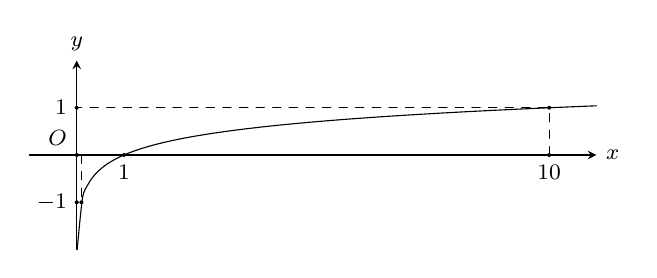
\begin{tikzpicture}[>=stealth,line join=round,line cap=round,font=\footnotesize,scale=0.6]
					\draw[->] (-1,0)--(11,0) node[right] {$x$};
					\draw[->] (0,-2)--(0,2) node[above] {$y$};
					\draw [smooth,domain=0.01:11,samples=100]plot(\x,{log10(\x)});
					\draw[dashed](10,0)--(10,1)--(0,1) (0.1,0)--(0.1,-1)--(0,-1);
					\fill (0,0)node[above left]{\footnotesize{$O$}}circle(1.2pt) (1,0)node[below]{\footnotesize{$1$}}circle(1.2pt) (10,0)node[below]{\footnotesize{$10$}}circle(1.2pt) (0,1)node[left]{\footnotesize{$1$}}circle(1.2pt) (0,-1)node[left]{\footnotesize{$-1$}}circle(1.2pt) (0.1,-1)circle(1.2pt) (10,1)circle(1.2pt);
				\end{tikzpicture}
			\end{center}
			\item Lập bảng giá trị của hàm số ta được
			\begin{center}
				\begin{tabular}{|c|c|c|c|c|c|}
					\hline
					$x$ & $\dfrac{1}{4}$ & $\dfrac{1}{2}$ & $1$ & $2$ & $4$ \\
					\hline
					$y=\log_{\tfrac{1}{4}}x$ & $1$ & $\dfrac{1}{2}$ & $0$ & $-\dfrac{1}{2}$ & $-1$\\
					\hline
				\end{tabular}
			\end{center}
			Đồ thị của hàm số $y=\log_{\tfrac{1}{4}}x$ như bên dưới
			\begin{center}
				\begin{tikzpicture}[>=stealth,line join=round,line cap=round,font=\footnotesize,scale=0.8]
					\draw[->] (-1,0)--(5,0) node[right] {$x$};
					\draw[->] (0,-2)--(0,2) node[above] {$y$};
					\draw [smooth,domain=0.065:5,samples=100]plot(\x,{(ln(\x))/(ln(0.25))});
					\draw[dashed](0.5,0)--(0.5,0.5)--(0,0.5) (4,0)--(4,-1)--(0,-1) (0.25,0)--(0.25,1)--(0,1);
					\fill (0,0)node[above left]{\footnotesize{$O$}}circle(1.2pt) (1,0)node[below]{\footnotesize{$1$}}circle(1.2pt) (4,0)node[above]{\footnotesize{$4$}}circle(1.2pt) (0.5,0)node[below]{\footnotesize{$\tfrac{1}{2}$}}circle(1.2pt) (0,1)node[left]{\footnotesize{$1$}}circle(1.2pt) (0,-1)node[left]{\footnotesize{$-1$}}circle(1.2pt) (0.5,0.5)circle(1.2pt) (4,-1)circle(1.2pt) (0.25,1)circle(1.2pt);
				\end{tikzpicture}
			\end{center}
	\end{enumEX}}
\end{bt}

\begin{bt}%[1D6H3-2]
% nguon: Archive/2024/TOAN_11_XE/TOAN_11_XE/data4/11C6/KNTT-6.3.tex #1001
%[Tex hóa SGK CD-CT,T7/22, TVN-019]
	Tìm tập xác định của các hàm số:
	\begin{enumEX}{2}
		\item $y=\log_2(3-2x)$.
		\item $y=\log_3\left(x^2+4x\right)$.
	\end{enumEX}
	\loigiai{\begin{enumerate}
			\item Hàm số $y=\log_2(3-2x)$ xác định khi $3-2x>0\Leftrightarrow x<\dfrac{3}{2}$.\\
			Vậy tập xác định của hàm số $y=\log_2(3-2x)$ là $\mathscr{D}=\left(-\infty;\dfrac{3}{2}\right)$.
			\item Hàm số $y=\log_3\left(x^2+4x\right)$ xác định khi $x^2+4x>0\Leftrightarrow x<-4\vee x>0$.\\
			Vậy tập xác định của hàm số $y=\log_3\left(x^2+4x\right)$ là $\mathscr{D}=(-\infty;-4)\cup(0;+\infty)$.
	\end{enumerate}}
\end{bt}

\begin{bt}%[1D6H3-2]
% nguon: Archive/2024/TOAN_11_XE/TOAN_11_XE/data4/11C6/KNTT-6.3.tex #1002
%[Đỗ Minh Phúc]
	Tìm tập xác định của các hàm số
	\begin{multicols}{3}
		\begin{enumerate}
			\item $y=12^x$;
			\item $y=\log_5(2 x-3)$;
			\item $y=\log_{\tfrac{1}{5}}\left(-x^2+4\right)$.
		\end{enumerate}
	\end{multicols}
	\loigiai{
		\begin{enumerate}
			\item Tập xác định của hàm số $y=12^x$ là $\mathscr{D}=\mathbb{R}$.
			\item Điều kiện $2x-3>0\Leftrightarrow x>\dfrac{3}{2}$.\\
			Vậy tập xác định của hàm số $y=\log_5(2x-3)$ là $\mathscr{D}=\left(\dfrac{3}{2};+\infty \right) $.
			\item Điều kiện $-x^2+4>0\Leftrightarrow -2<x<2$.\\
			Vậy tập xác định của hàm số $y=\log_{\tfrac{1}{5}}\left(-x^2+4\right)$ là $\mathscr{D}=(-2;2)$.
		\end{enumerate}
	}
\end{bt}

\begin{bt}%[1D6H3-5]
% nguon: Archive/2024/TOAN_11_XE/TOAN_11_XE/data4/11C6/KNTT-6.3.tex #1003
%[Tex hóa SGK CD-CT,T7/22, TVN-019]
	Cường độ ánh sáng $I$ dưới mặt biển giảm dần theo độ sâu theo công thức $I=I_0\cdot a^d$, trong đó $I_0$ là cường độ ánh sáng tại mặt nước biển, $a>0$ là hằng số và $d$ là độ sâu tính bằng mét tính từ mặt nước biển.
	\begin{center}
		(\textit{Nguồn:}  http://www.britannica.com/science/seawer/Optical-properties)
	\end{center}
	\begin{enumerate}
		\item Có thể khẳng định rằng $0<a<1$ không? Giải thích.
		\item Biết rằng cường độ ánh sáng tại độ sâu $1$m bằng $0{,}95I_0$. Tìm giá trị của $a$.
		\item Tại độ sâu $20$m, cường độ ánh sáng bằng bao nhiêu phần trăm so với $I_0$? (Làm tròn kết quả đến hàng đơn vị.)
	\end{enumerate}
	\loigiai{\begin{enumerate}
			\item Do $I_0$ là cường độ ánh sáng tại mặt nước biển là không đổi, nên cường độ ánh sáng $I$ tỉ lệ thuận với hàm số $a^d$.\\
			Do $I$ giảm dần theo độ sâu, nên hàm số $a^d$ nghịch biến, suy ra $0<a<1$.
			\item Tại độ sâu $1$m, ta có cường độ ánh sáng $I=0{,}95I_0$, suy ra $0{,}95I_0=I_0a^1\Leftrightarrow a=0{,}95$.
			\item Tại độ sâu $20$m, suy ra $d=20$. Cường độ ánh sáng tại đó là $I=I_0a^d=I_0\cdot0{,}95^{20}\approx0{,}4I_0$.\\
			Vậy tại độ sâu $20$m, cường độ ánh sáng tại đó bằng khoảng $40$\% so với $I_0$.
	\end{enumerate}}
\end{bt}

\begin{bt}%[1D6H3-3]
% nguon: Archive/2024/TOAN_11_XE/TOAN_11_XE/data4/11C6/KNTT-6.3.tex #1005
%[Đỗ Minh Phúc]
	Lập bảng biến thiên và vẽ đồ thị hàm số
	\begin{multicols}{2}
		\begin{enumerate}
			\item $y=4^x$;
			\item $y=\log_{\tfrac{1}{4}} x$.
		\end{enumerate}
	\end{multicols}
	\loigiai{
		\begin{enumerate}
			\item 	Vì hàm số $y=4^x$ có cơ số $4>1$ nên ta có bảng biến thiên như sau
			\begin{center}
				\begin{tikzpicture}[>=stealth,line join=round,line cap=round,font=\footnotesize,scale=1]
					\tkzTabInit[nocadre=false,lgt=2,espcl=2,deltacl=0.5]{$x$/0.7,$y=4^x$/2}
					{$-\infty$ , $0$ , $+\infty$}
					\tkzTabVar{-/$0$ , R , +/$+\infty$}
					\tkzTabIma{1}{3}{2}{$1$}% Từ cột 1 đến cột 3 đặt f(2) tại cột 2.
				\end{tikzpicture}
			\end{center}
			Đồ thị của hàm số $y=4^x$ là một đường cong liền nét đi qua các điểm $A\left(-1;\dfrac{1}{4}\right)$, $B(0;1)$, $C(1;4)$, $D(2;16)$.
			\begin{center}
				\begin{tikzpicture}[>=stealth,line join=round,line cap=round,font=\footnotesize,scale=0.8,yscale=0.7]
					\def\a{4}
					\draw[->] (-3.5,0) -- (5,0) node[below] {$x$};
					\draw[->] (0,-2) -- (0,17) node[left] {$y$};
					\draw (0,0)node[below right=-0.05]{$O$};
					\clip (-5,-5)rectangle(5,16.5);
					\draw[thick,samples=200,smooth,domain=-3:4] plot(\x, {\a^\x});
					\draw[dashed] (0,4)--(1,4) node[right]{$C$}--(1,0);
					\draw[dashed] (0,16)--(2,16)node[right]{$D$}--(2,0);
					\draw[dashed] (-1,0)--(-1,1/4)node[above left]{$A$}--(0,1/4)node[right]{$\frac{1}{4}$};
					\draw (0,1) node [above left=-0.1] {$1$}node[right]{$B$};
					\draw (1,0) node [below] {$1$};
					\draw (0,4) node [left] {$4$};
					\draw (2,0) node [below] {$2$};
					\draw (0,16) node [left] {$16$};
					\draw (-1,0) node [below] {$-1$};
				\end{tikzpicture}
			\end{center}
			\item Vì hàm số $y=\log_{\tfrac{1}{4}} x$ có cơ số $\dfrac{1}{4}<1$ nên ta có bảng biến thiên như sau
			\begin{center}
				\begin{tikzpicture}[>=stealth,line join=round,line cap=round,font=\footnotesize,scale=1]
					\tkzTabInit[nocadre=true,lgt=2.3,espcl=2,deltacl=0.5]{$x$/0.7,$y=\log_{\tfrac{1}{4}}x$/2}
					{$0$ , $1$ , $+\infty$}
					\tkzTabVar{+/$+\infty$ , R , -/$-\infty$}
					\tkzTabIma{1}{3}{2}{$0$}% Từ cột 1 đến cột 3 đặt f(2) tại cột 2.
				\end{tikzpicture}
			\end{center}
			Đồ thị của hàm số $y=\log_{\tfrac{1}{4}}x$ là một đường cong liền nét đi qua các điểm $A\left(\dfrac{1}{4};1\right)$, $B(1;0)$, $C(4;-1)$, $D(16;-2)$.
			\begin{center}
				\begin{tikzpicture}[>=stealth,line join=round,line cap=round,font=\footnotesize,scale=0.9,xscale=0.8]
					\draw[->](-1,0) -- (17,0) node[below]{ $x$};
					\draw[->](0,-3) -- (0,4) node[below,right]{ $y$};
					\draw(-0.2,0) node[below left]{\footnotesize $O$};
					\clip(-2,-3) rectangle (17,4);
					\draw[smooth,samples=300,domain=0.03:16.5]plot(\x,{ln(\x)/ln(0.25)});
					\draw(1,0) node[below]{$1$}node[above]{$B$};
					\draw[dashed] (0,-1) node[left]{$-1$}--(4,-1)node[below]{$C$}--(4,0)node[above]{$4$};
					\draw[dashed] (0,-2) node[left]{$-2$}--(16,-2)node[below]{$D$}--(16,0)node[above]{$16$};
					\draw[dashed] (0,1) node[left]{$1$}--(1/4,1)node[right]{$A$}--(1/4,0)node[below]{$\frac{1}{4}$};
					\draw (0.1,2)node[right]{$y=\log_{\tfrac{1}{4}}x$};
				\end{tikzpicture}
			\end{center}
		\end{enumerate}
	}	
\end{bt}

\begin{bt}%[1D6H3-3]
% nguon: Archive/2024/TOAN_11_XE/TOAN_11_XE/data4/11C6/KNTT-6.3.tex #1006
%[Đỗ Minh Phúc]
	Trong các hàm số sau, hàm số nào đồng biến, hàm số nào nghịch biến trên khoảng xác định của hàm số đó? Vì sao?
	\begin{multicols}{4}
		\begin{enumerate}
			\item $y=\left(\dfrac{\sqrt{3}}{2}\right)^x$;
			\item $y=\left(\dfrac{\sqrt[3]{26}}{3}\right)^x$;
			\item $y=\log_\pi x$;
			\item $y=\log_{\tfrac{\sqrt{15}}{4}} x$.
		\end{enumerate}
	\end{multicols}
	\loigiai{
		\begin{enumerate}
			\item Vì $0<\dfrac{\sqrt{3}}{2}<1$ nên hàm số $y=\left(\dfrac{\sqrt{3}}{2}\right)^x$ nghịch biến trên $\mathbb{R}$.
			\item Vì $0<\dfrac{\sqrt{3}}{2}<1$ nên hàm số $y=\left(\dfrac{\sqrt[3]{26}}{3}\right)^x$ nghịch biến trên $\mathbb{R}$.
			\item Vì $\pi>1$ nên hàm số $y=\log_\pi x$ đồng biến trên $(0;+\infty)$.
			\item Vì $0<\tfrac{\sqrt{15}}{4}<1$ nên hàm số $y=\log_{\tfrac{\sqrt{15}}{4}} x$ nghịch biến trên $(0;+\infty)$.
		\end{enumerate}	
	}
\end{bt}

\begin{bt}%[1D6H3-5]
% nguon: Archive/2024/TOAN_11_XE/TOAN_11_XE/data4/11C6/KNTT-6.3.tex #1007
%[Đỗ Minh Phúc]
	Ta coi năm lấy làm mốc để tính dân số của một vùng (hoặc một quốc gia) là năm 0. Khi đó, dân số của quốc gia đó ở năm thứ $t$ là hàm số theo biến $t$ được cho bởi công thức: $S=A \cdot e^{rt}$. Trong đó $A$ là dân số của vùng (hoặc quốc gia) đó ở năm 0 và $r$ là tỉ lệ tăng dân số hằng năm (Nguồn: Giải tích 12, NXBGD Việt Nam, 2021). Biết rằng dân số Việt Nam năm 2021 ước tính là $98564407$ người và tỉ lệ tăng dân số $0,93\%$/năm (Nguồn: https://danso.org/viet-nam). Giả sử tỉ lệ tăng dân số hằng năm là như nhau tính từ năm 2021, nêu dự đoán dân số Việt Nam năm 2030 (làm tròn kết quả đến hàng đơn vị).
	\loigiai{
		Dân số Việt Nam vào năm 2030 là
		$$S=A \cdot e^{rt}=98564407\cdot e^{0,93\%\cdot 9}\approx 107169341\text{ (người).}$$
	}
\end{bt}

\begin{bt}%[1D6H3-5]
% nguon: Archive/2024/TOAN_11_XE/TOAN_11_XE/data4/11C6/KNTT-6.3.tex #1008
%[Đỗ Minh Phúc]
	Các nhà tâm lí học sử dụng mô hình hàm số mũ để mô phỏng quá trình học tập của một học sinh như sau: $f(t)=c\left(1-e^{-k t}\right)$, trong đó $c$ là tổng số đơn vị kiến thức học sinh phải học, $k$ (kiến thức/ngày) là tốc độ tiếp thu của học sinh, $t$ (ngày) là thời gian học và $f(t)$ là số đơn vị kiến thức học sinh đã học được (Nguồn: R.I. Charles et al., Algebra 2, Pearson). Giả sử một em học sinh phải tiếp thu $25$ đơn vị kiến thức mới. Biết rằng tốc độ tiếp thu của em học $\sinh$ là $k=0{,}2$. Hỏi em học sinh sẽ nhớ được (khoảng) bao nhiêu đơn vị kiến thức mới sau $2$ ngày? Sau $8$ ngày?
	\loigiai{
		Số đơn vị kiến thức mới em học sinh sẽ nhớ sau $2$ ngày là
		$$f(2)=25\left(1-e^{-0{,}2\cdot2}\right)\approx 8{,}24\text{ (đơn vị)}.$$
		Số đơn vị kiến thức mới em học sinh sẽ nhớ sau $8$ ngày là
		$$f(8)=25\left(1-e^{-0{,}2\cdot8}\right)\approx 19{,}95\text{ (đơn vị)}.$$
	}	
\end{bt}

\begin{bt}%[1D6H3-5]
% nguon: Archive/2024/TOAN_11_XE/TOAN_11_XE/data4/11C6/KNTT-6.3.tex #1009
%[Đỗ Minh Phúc]
	Chỉ số hay độ pH của một dung dịch được tính theo công thức: $\mathrm{pH}=-\log \left[\mathrm{H}^{+}\right]$. Phân tích nồng độ ion hydrogen $\left[\mathrm{H}^{+}\right]$ trong hai mẫu nước sông, ta có kết quả sau: Mẫu 1: $\left[\mathrm{H}^{+}\right]=8 \cdot 10^{-7}$; Mẫu $2:\left[\mathrm{H}^{+}\right]=2 \cdot 10^{-9}$.
	Không dùng máy tính cầm tay, hãy so sánh độ pH của hai mẫu nước trên.
	\loigiai{
		Hàm số $\mathrm{pH}=-\log \left[\mathrm{H}^{+}\right]$ có $a=10>1$ nên nghịch biến trên $(0;+\infty)$.\\
		Vì $8 \cdot 10^{-7}>2 \cdot 10^{-9}$ nên độ pH của mẫu 1 bé hơn độ pH của mẫu 2.
	}
\end{bt}

\begin{bt}%[1D6H2-4]
% nguon: Archive/2024/TOAN_11_XE/TOAN_11_XE/data4/11C6/KNTT-6.3.tex #1010
%[Đỗ Minh Phúc]
	Một người gửi $10$ triệu đồng vào ngân hàng theo hình thức lãi kép có kì hạn là 12 tháng vối lãi suất $6\%$/năm. Giả sử qua các năm thì lãi suất không thay đổi và người đó không gửi thêm tiền vào mỗi năm. Để biết sau $y$ (năm) thì tổng số tiền cả vốn và lãi có được là $x$ (đồng), người đó sử dụng công thức $y=\log_{1,06}\left(\dfrac{x}{10}\right)$. Hỏi sau bao nhiêu năm thì người đó có được tổng số tiền cả vốn và lãi là $15$ triệu đồng? $20$ triệu đồng? (Làm tròn kết quả đến hàng đơn vị).
	\loigiai{
		Người đó có được tổng số tiền cả vốn lẫn lãi là $15$ triệu đồng sau
		$$y=\log_{1,06}\left(\dfrac{15}{10}\right)\approx 7\text{ (năm).}$$
		Người đó có được tổng số tiền cả vốn lẫn lãi là $20$ triệu đồng sau
		$$y=\log_{1,06}\left(\dfrac{20}{10}\right)\approx 12\text{ (năm).}$$
	}
\end{bt}

\begin{bt}%[1D6H1-4]
% nguon: Archive/2024/TOAN_11_XE/TOAN_11_XE/data4/11C6/KNTT-6.3.tex #1011
%[Tex hóa SGK CD-CT,T7/22, TVN-019]
	So sánh các cặp số sau:
	\begin{enumEX}{2}
		\item $1{,}3^{0{,}7}$ và $1{,}3^{0{,}6}$.
		\item $0{,}75^{-2{,}3}$ và $0{,}75^{-2{,}4}$.
	\end{enumEX}
	\loigiai{\begin{enumerate}
			\item Do $1{,}3>1$ nên hàm số $y=1{,}3^x$ đồng biến trên $\mathbb{R}$. Mà $0{,}7>0{,}6$ nên $1{,}3^{0{,}7}>1{,}3^{0{,}6}$.
			\item Do $0{,}75<1$ nên hàm số $y=0{,}75^x$ nghịch biến trên $\mathbb{R}$. Mà $-2{,}3>-2{,}4$ nên $0{,}75^{-2{,}3}<0{,}75^{-2{,}4}$.
	\end{enumerate}}
\end{bt}

\begin{bt}%[1D6H3-4]
% nguon: Archive/2024/TOAN_11_XE/TOAN_11_XE/data4/11C6/KNTT-6.3.tex #1012
%[Tex hóa SGK CD-CT,T7/22, TVN-019]
	So sánh các cặp số sau:
	\begin{enumEX}{2}
		\item $\log_{\pi}0{,}8$ và $\log_{\pi}1{,}2$.
		\item $\log_{0{,}3}2$ và $\log_{0{,}3}2{,}1$.
	\end{enumEX}
	\loigiai{\begin{enumerate}
			\item Hàm số $y=\log_{\pi}x$ có cơ số $\pi>1$ nên đồng biến trên $(0;+\infty)$.\\
			Mà $0{,}8<1{,}2$ nên $\log_{\pi}0{,}8<\log_{\pi}1{,}2$.
			\item Hàm số $y=\log_{0{,}3}x$ có cơ số $0{,}3<1$ nên nghịch biến trên $(0;+\infty)$.\\
			Mà $2<2{,}1$ nên $\log_{0{,}3}2>\log_{0{,}3}2{,}1$.
	\end{enumerate}}
\end{bt}

\begin{bt}%[1D6N4-2]
% nguon: Archive/2024/TOAN_11_XE/TOAN_11_XE/data4/11C6/KNTT-6.4.tex #1013
%[TeX hóa SGK 11 - CTST - Đoàn Mạnh Hùng]
	Giải các phương trình sau
	\begin{listEX}[3]
		\item $2^x=\dfrac{1}{8}$.
		\item $5\cdot 10^x=1$.
		\item $\left(\dfrac{1}{9}\right)^x=\dfrac{27^x}{3}$.
	\end{listEX}
	\loigiai{
		\begin{listEX}[1]
			\item $2^x=\dfrac{1}{8} \Leftrightarrow 2^x=2^{-3} \Leftrightarrow x=-3$.
			\item $5 \cdot 10^x=1 \Leftrightarrow 10^x=\dfrac{1}{5} \Leftrightarrow x=\log \dfrac{1}{5}=-\log 5$.
			\item 
			\allowdisplaybreaks
			\begin{eqnarray*}
				&&\left(\dfrac{1}{9}\right)^x=\dfrac{27^x}{3} \Leftrightarrow\left(3^{-2}\right)^x=\dfrac{\left(3^3\right)^x}{3} \Leftrightarrow 3^{-2 x}=3^{3 x-1}\\
				&\Leftrightarrow&-2 x=3 x-1 \Leftrightarrow 5 x=1 \Leftrightarrow x=\dfrac{1}{5}.
			\end{eqnarray*}
		\end{listEX}
	}
\end{bt}

\begin{bt}%[1D6H4-2]
% nguon: Archive/2024/TOAN_11_XE/TOAN_11_XE/data4/11C6/KNTT-6.4.tex #1014
%[TeX hóa SGK 11 - CTST - Đoàn Mạnh Hùng]
	Giải các phương trình sau
	\begin{listEX}[3]
		\item $3^{x+2}=\sqrt[3]{9}$.
		\item $2\cdot 10^{2 x}=30$.
		\item $4^{2 x}=8^{2 x-1}$.
	\end{listEX}
	\loigiai{
		\begin{listEX}
			\item $3^{x+2}=\sqrt[3]{9}\Leftrightarrow x+2=\dfrac{2}{3}\Leftrightarrow x=-\dfrac{4}{3}$.
			\item $2\cdot 10^{2 x}=30\Leftrightarrow x=\dfrac{1}{2}\log_{10} 15$.
			\item $4^{2 x}=8^{2 x-1}\Leftrightarrow 2^{4x}=2^{6x-3}\Leftrightarrow x=\dfrac{3}{2}$.
		\end{listEX}
	}
\end{bt}

\begin{bt}%[1D6N4-2]
% nguon: Archive/2024/TOAN_11_XE/TOAN_11_XE/data4/11C6/KNTT-6.4.tex #1015
%[TeX hóa SGK 11 - CTST - Đoàn Mạnh Hùng]
	Giải các phương trình sau
	\begin{listEX}[2]
		\item $\log _3 x=-2$.
		\item $\log _2\left(x^2-3\right)=\log _2 2 x$.
	\end{listEX}
	\loigiai{
		\begin{listEX}
			\item Điều kiện: $x>0$.\\
			$\log_3 x=-2 \Leftrightarrow x=3^{-2}=\dfrac{1}{3^2}=\dfrac{1}{9}$.
			\item Điều kiện: $\heva{&x^2-3>0 \\ &2x>0}$ (*)\\
			Khi đó, phương trình đã cho trở thành $x^2-3=2 x \Leftrightarrow x^2-3-2 x=0 \Leftrightarrow x=-1$ hoặc $x=3$.\\
			Thay lần lượt hai giá trị này vào (*), ta thấy chỉ có $x=3$ thoả mãn.\\
			Vậy phương trình có nghiệm là $x=3$.
		\end{listEX}
	}
\end{bt}

\begin{bt}%[1D6H4-2]
% nguon: Archive/2024/TOAN_11_XE/TOAN_11_XE/data4/11C6/KNTT-6.4.tex #1016
%[TeX hóa SGK 11 - CTST - Đoàn Mạnh Hùng]
	Giải các phương trình sau
	\begin{listEX}[2]
		\item $\log _{\tfrac{1}{2}}(x-2)=-2$.
		\item $\log _2(x+6)=\log _2(x+1)+1$.
	\end{listEX}
	\loigiai{
		\begin{listEX}[1]
			\item Điều kiện: $x>2$.\\
			$\log _{\tfrac{1}{2}}(x-2)=-2\Leftrightarrow x-2=4\Leftrightarrow x=6$.
			\item Điều kiện: $\heva{&x>-6\\&x>-1}\Leftrightarrow x>-1$.\\
			$\log _2(x+6)=\log _2(x+1)+1\Leftrightarrow \log _2(x+6)=\log _2(2x+2)\Leftrightarrow x+6=2x+2\Leftrightarrow x=4$.
		\end{listEX}
	}
\end{bt}

\begin{bt}%[1D6N4-3]
% nguon: Archive/2024/TOAN_11_XE/TOAN_11_XE/data4/11C6/KNTT-6.4.tex #1017
%[TeX hóa SGK 11 - CTST - Đoàn Mạnh Hùng]
	Giải các bất phương trình sau
	\begin{listEX}[3]
		\item $10^x<0{,}001$.
		\item $0{,}4^x>2$.
		\item $\left(\dfrac{1}{2}\right)^x \geq 2 \cdot 4^{2x}$.
	\end{listEX}
	\loigiai{
		\begin{listEX}[1]
			\item $10^x<0{,}001 \Leftrightarrow 10^x<10^{-3} \Leftrightarrow x<-3$ (do $10>1$ ).
			\item $0{,}4^x>2 \Leftrightarrow x<\log _{0{,}4} 2$ (do $0<0{,}4<1)$.
			\item
			\allowdisplaybreaks
			\begin{eqnarray*}
				&&\left(\dfrac{1}{2}\right)^x \geq 2 \cdot 4^{2 x}  \Leftrightarrow\left(2^{-1}\right)^x \geq 2 \cdot\left(2^2\right)^{2 x} \Leftrightarrow 2^x \geq 2^{1+4 x} \\
				&\Leftrightarrow&-x \geq 1+4 x \Leftrightarrow 5 x \leq-1 \Leftrightarrow x \leq-\dfrac{1}{5}.
			\end{eqnarray*}
		\end{listEX}
	}
\end{bt}

\begin{bt}%[1D6N4-3]
% nguon: Archive/2024/TOAN_11_XE/TOAN_11_XE/data4/11C6/KNTT-6.4.tex #1018
%[TeX hóa SGK 11 - CTST - Đoàn Mạnh Hùng]
	Giải các bất phương trình sau
	\begin{listEX}[3]
		\item $2^x>16$.
		\item $0{,}1^x \leq 0{,}001$.
		\item $\left(\dfrac{1}{5}\right)^{x-2} \geq\left(\dfrac{1}{25}\right)^x$.
	\end{listEX}
	\loigiai{
		\begin{listEX}[1]
			\item $2^x>16\Leftrightarrow x>4$.
			\item $0{,}1^x \leqslant  0{,}001\Leftrightarrow 0{,}1^x \leqslant  0{,}1^3\Leftrightarrow x\geqslant 3$.
			\item $\left(\dfrac{1}{5}\right)^{x-2} \geqslant \left(\dfrac{1}{25}\right)^x\Leftrightarrow \left(\dfrac{1}{5}\right)^{x-2}\geqslant \left(\dfrac{1}{5}\right)^{2x}\Leftrightarrow x-2\leqslant 2x\Leftrightarrow x\geqslant -2$.
		\end{listEX}
	}
\end{bt}

\begin{bt}%[1D6H4-3]
% nguon: Archive/2024/TOAN_11_XE/TOAN_11_XE/data4/11C6/KNTT-6.4.tex #1019
%[TeX hóa SGK 11 - CTST - Đoàn Mạnh Hùng]
	Giải các bất phương trình sau
	\begin{listEX}[2]
		\item $\log _2(2 x-1) \leqslant  1$.
		\item $\log _{\tfrac{1}{2}}(1-x)>\log _{\tfrac{1}{2}}(3 x+2)$.
	\end{listEX} 
	\loigiai{
		\begin{listEX}[1]
			\item Điều kiện: $2 x-1>0 \Leftrightarrow x>\dfrac{1}{2}$.\\
			Khi đó, do cơ số $2>1$ nên bất phương trình đã cho trở thành
			$$2 x-1 \leq 2^{1} \Leftrightarrow 2 x \leqslant 3 \Leftrightarrow x \leqslant \dfrac{3}{2}.$$
			Vậy nghiệm của bất phương trình là $\dfrac{1}{2}<x \leqslant  \dfrac{3}{2}$.
			\item Điều kiện: $\heva{&1-x>0 \\& 3 x+2>0} \Leftrightarrow\heva{&x<1 \\& x>-\dfrac{2}{3}} \Leftrightarrow-\dfrac{2}{3}<x<1$. (*)\\
			Khi đó, do cơ số $\frac{1}{2}<1$ nên bất phương trình đã cho trở thành
			$$1-x<3 x+2 \Leftrightarrow 4 x>-1 \Leftrightarrow x>-\dfrac{1}{4}.$$
			Kết hợp với điều kiện $(*)$, ta được nghiệm của bất phương trình là $-\dfrac{1}{4}<x<1$.
		\end{listEX}
	}
\end{bt}

\begin{bt}%[1D6N4-3]
% nguon: Archive/2024/TOAN_11_XE/TOAN_11_XE/data4/11C6/KNTT-6.4.tex #1020
%[TeX hóa SGK 11 - CTST - Đoàn Mạnh Hùng]
	Giải các bất phương trình sau
	\begin{listEX}[2]
		\item $\log _{\tfrac{1}{3}}(x+1)<2$.
		\item $\log _5(x+2) \leq 1$.
	\end{listEX}
	\loigiai{
		\begin{listEX}[1]
			\item Điều kiện: $x>-1$.\\
			$\log _{\tfrac{1}{3}}(x+1)<2\Leftrightarrow x+1>\left(\dfrac{1}{3}\right)^2\Leftrightarrow x>-\dfrac{8}{9}$.\\
			Vậy nghiệm của bất phương trình là $x>-\dfrac{8}{9}$
			\item Điều kiện $x>-2$.\\
			$\log _5(x+2) \leq 1\Leftrightarrow x+2\le 5\Leftrightarrow x\le 3$.\\
			Vậy nghiệm của bất phương trình là $-2<x\le 3$.
	\end{listEX}}
\end{bt}

\begin{bt}%[1D6V4-6]
% nguon: Archive/2024/TOAN_11_XE/TOAN_11_XE/data4/11C6/KNTT-6.4.tex #1021
%[TeX hóa SGK 11 - CTST - Đoàn Mạnh Hùng]
	Nước chanh có độ pH bằng $2{,}4$; giấm có độ pH bằng $3$. Nước chanh có độ acid gấp bao nhiêu lần giấm (nghĩa là có nồng độ H$^{+}$ gấp bao nhiêu lần)? (Làm tròn kết quả đến hàng phần trăm).
	\loigiai{
		Kí hiệu $x, y$ lần lượt là nồng độ H$^{+}$ trong nước chanh và giấm.\\ Theo giả thiết, ta có $2{,}4=-\log x$ và $3=-\log y$.\\
		Suy ra $x=10^{-2{,}4}$ và $y=10^{-3}$. Suy ra $\dfrac{x}{y}=\dfrac{10^{-2{,}4}}{10^{-3}}=10^{0{,}6} \approx 3{,}98$.\\
		Vậy nồng độ H$^{+}$ của nước chanh gấp $3{,}98$ lần nồng độ H$^{+}$ của giấm.
	}
\end{bt}

\begin{bt}%[1D6H4-6]
% nguon: Archive/2024/TOAN_11_XE/TOAN_11_XE/data4/11C6/KNTT-6.4.tex #1022
%[TeX hóa SGK 11 - CTST - Đoàn Mạnh Hùng]
	Nước uống đạt tiêu chuẩn phải có độ $\mathrm{pH}$ nằm trong khoảng từ $6{,}5$ đến $8{,}5$ (theo Quy chuẩn Việt Nam QCVN $01: 2009 / \mathrm{BYT}$ ). Nồng độ $\mathrm{H}^{+}$ trong nước uống tiêu chuẩn phải nằm trong khoảng nào?
	\loigiai{
		Gọi $x$ là nồng độ $\mathrm{H}^{+}$ trong nước. Ta có
		$$-\log 6{,}5<x<-\log 8{,}5\Leftrightarrow -0{,}813<x<-0{,}924.$$
	}
\end{bt}

\begin{bt}%[1D6V4-6]
% nguon: Archive/2024/TOAN_11_XE/TOAN_11_XE/data4/11C6/KNTT-6.4.tex #1023
%[TeX hóa SGK 11 - CTST - Đoàn Mạnh Hùng]
	Công thức tính khối lượng còn lại của một chất phóng xạ từ khối lượng ban đầu $M_0$ là $M(t)=M_0\left(\dfrac{1}{2}\right)^{\tfrac{1}{T}}$, trong đó $t$ là thời gian tính từ thời điểm ban đầu và $T$ là chu kì bán rã của chất. Đồng vị plutonium-$234$ có chu kì bán rã là $9$ giờ.
	\begin{flushright}
		(\textit{Nguồn: https://pubchem.ncbi.nlm.nih.gov/element/Plutonium\#section=AtomicMass\\-Half-Life-and-Deca})
	\end{flushright}
	Từ khối lượng ban đầu $200 \mathrm{~g}$, sau bao lâu thì khối lượng plutonium-$234$ còn lại là
	\begin{listEX}[3]
		\item $100 \mathrm{~g}$?
		\item $50 \mathrm{~g}$?
		\item $20 \mathrm{~g}$?
	\end{listEX}
	\loigiai{
		\begin{listEX}
			\item $100 =200\left(\dfrac{1}{2}\right)^{\tfrac{t}{9}}\Leftrightarrow t=9$ giờ.
			\item $50=200\left(\dfrac{1}{2}\right)^{\tfrac{t}{9}}\Leftrightarrow t=18$ giờ.
			\item $20=200\left(\dfrac{1}{2}\right)^{\tfrac{t}{9}}\Leftrightarrow t=9\cdot \log_{\tfrac{1}{2}} \dfrac{1}{10} \approx 29{,}9$ giờ.
		\end{listEX}	
	}
\end{bt}

\begin{bt}%[1D6H4-4]
% nguon: Archive/2024/TOAN_11_XE/TOAN_11_XE/data4/11C6/KNTT-6.4.tex #1025

	Giải mỗi phương trình sau
	\begin{listEX}[2]
		\item $(0{,}3)^{x-3}=1$;
		\item $5^{3x-2}=25$;
		\item $9^{x-2}=243^{x+1}$;
		\item $\log_{\frac{1}{2}} (x+1)=-3$;
		\item $\log_5 (3x-5) =\log_5 (2x+1)$;
		\item $\log_{\frac{1}{7}}(x+9)=\log_{\frac{1}{7}} (2x-1)$.
	\end{listEX}
	\loigiai{
		Ta có
		\begin{enumerate}
			\item  $(0{,}3)^{x-3}=1 \Leftrightarrow x-3=\log_{0{,}3} 1\Leftrightarrow x-3=0 \Leftrightarrow x=3$.\\
			Vậy phương trình có nghiệm là $x=3$.
			\item  $5^{3x-2}=25 \Leftrightarrow 3x-2=\log_5 25 \Leftrightarrow 3x-2=2 \Leftrightarrow 3x=4 \Leftrightarrow x=\dfrac{4}{3}$.\\
			Vậy phương trình có nghiệm là $x=\dfrac{4}{3}$.
			\item  Ta có
			\begin{eqnarray*}
				9^{x-2}=243^{x+1} &\Leftrightarrow& 3^{2(x-2)} = 3^{5(x+1)}\\
				&\Leftrightarrow& 2(x-2)=5(x+1) \\
				&\Leftrightarrow& 2x-4=5x+5\\
				&\Leftrightarrow& -3x=9 \\
				&\Leftrightarrow& x=-3.
			\end{eqnarray*}
			Vậy phương trình có nghiệm là $x=-3$.
			\item $\log_{\frac{1}{2}} (x+1)=-3 \Leftrightarrow x+1=\left(\dfrac{1}{2}\right)^{-3} \Leftrightarrow x+1=8 \Leftrightarrow x=7$.\\
			Vậy phương trình có nghiệm là $x=7$.
			\item   $\log_5 (3x-5) =\log_5 (2x+1)$\\
			Điều kiện: $
			\heva{
				&3x-5>0\\
				&2x+1>0
			}\Leftrightarrow \heva{
				&x>\dfrac{5}{3}\\
				&x>-\dfrac{1}{2}
			} \Leftrightarrow x>\dfrac{5}{3}.
			$\\
			Phương trình đã cho $\log_5 (3x-5) =\log_5 (2x+1)$
			\[
			\Leftrightarrow 
			\heva{
				&x>\dfrac{5}{3}\\
				&3x-5=2x+1
			} \Leftrightarrow
			\heva{
				&x>\dfrac{5}{3}\\
				&x=6
			} \Leftrightarrow x=6.\]
			Vậy phương trình có nghiệm là $x=6$.
			\item  Phương trình $\log_{\frac{1}{7}}(x+9)=\log_{\frac{1}{7}} (2x-1)
			\Leftrightarrow 
			\heva{
				&x+9>0\\
				&x+9=2x-1
			} \Leftrightarrow
			\heva{
				&x>-9\\
				&x=10
			} \Leftrightarrow x=10.
			$\\
			Vậy phương trình có nghiệm là $x=10$.
		\end{enumerate}
	}
\end{bt}

\begin{bt}%[1D6H4-5]
% nguon: Archive/2024/TOAN_11_XE/TOAN_11_XE/data4/11C6/KNTT-6.4.tex #1026

	Giải mỗi bất phương trình sau
	\begin{listEX}[2]
		\item $3^x>\dfrac{1}{243}$;
		\item $\left(\dfrac{2}{3}\right)^{3x-7}\leq \dfrac{3}{2}$;
		\item $4^{x+3}\geq 32^x$;
		\item $\log (x-1)<0$;
		\item $\log_{\frac{1}{2}}(2x-1)\geq \log_{\frac{1}{2}} (x+3)$;
		\item $\ln (x+3)\geq \ln (2x-8)$.
	\end{listEX}
	\loigiai{
		Ta có
		\begin{enumerate}
			\item  $3^x>\dfrac{1}{243} \Leftrightarrow x>\log_3 \dfrac{1}{243} \Leftrightarrow x>-5$.\\
			Vậy tập nghiệm của bất phương trình là $(-5;+\infty)$.
			\item  $\left(\dfrac{2}{3}\right)^{3x-7}\leq \dfrac{3}{2}
			\Leftrightarrow 3x-7 \geq \log_{\frac{2}{3}} \dfrac{3}{2}\Leftrightarrow 3x\geq 6 \Leftrightarrow x\geq  2$.\\
			Vậy tập nghiệm của bất phương trình là $[2;+\infty)$.
			\item  $4^{x+3}\geq 32^x \Leftrightarrow 2^{2(x+3} \geq 2^{5x} \Leftrightarrow 2(x+3)\geq 5x \Leftrightarrow -3x \geq -6 \Leftrightarrow x\leq 2$.\\
			Vậy tập nghiệm của bất phương trình là $(-\infty;2]$.
			\item   $\log (x-1)<0 \Leftrightarrow \heva{
				&x-1>0\\
				&x-1<10^0
			} \Leftrightarrow \heva{
				&x>1\\
				&x<2
			} \Leftrightarrow 1<x<2$.\\
			Vậy tập nghiệm của bất phương trình là $(1;2)$.
			\item  Bất phương trình $\log_{\frac{1}{2}}(2x-1)\geq \log_{\frac{1}{2}} (x+3)$
			\[
			\Leftrightarrow \heva{
				&2x-1>0\\
				& 2x-1 \leq x+3
			} \Leftrightarrow 
			\heva{
				&x>\dfrac{1}{2}\\
				&x\leq  4
			} \Leftrightarrow \dfrac{1}{2}<x\leq 4.
			\]
			Vậy tập nghiệm của bất phương trình là $\left(\dfrac{1}{2};4\right]$.
			\item  $\ln (x+3)\geq \ln (2x-8) \Leftrightarrow
			\heva{
				&2x-8>0\\
				&x+3\geq 2x-8
			}\Leftrightarrow
			\heva{
				&x>4\\
				&x\leq 11
			} \Leftrightarrow 4<x\leq 11
			$.\\
			Vậy tập nghiệm của bất phương trình là $\left(4;11\right]$.
		\end{enumerate}
	}
\end{bt}

\begin{bt}%[1D6V4-6]
% nguon: Archive/2024/TOAN_11_XE/TOAN_11_XE/data4/11C6/KNTT-6.4.tex #1027

	Một người gửi ngân hàng $100$ triệu đồng theo hình thức lãi kép có kì hạn là $12$ tháng với lãi suất là $x$ $\%$/năm ($x>0$). Sau $3$ năm, người đó rút được cả gốc và lãi là $119{,}1016$ triệu đồng. Tìm $x$, biết rằng lãi suất không thay đổi qua các năm và người đó không rút tiền ra trong suốt thời gian gửi.
	\loigiai{
		Gọi $P_n$ là số tiền gốc và lãi nhận được sau $n$ kì gửi.\\
		$P_0$ là số tiền gửi ban đầu.\\
		$x\%$ lãi suất.\\
		Với $n=3$ năm, $P_3=119{,}1016$ triệu; $P_0=100$ triệu, ta có 
		\[
		P_3=P_0(1+x)^3 \Leftrightarrow (1+x)^3=\dfrac{P_3}{P_0} \Leftrightarrow
		1+x=\sqrt[3]{\dfrac{P_3}{P_0}} \]
		\[\Leftrightarrow x=\sqrt[3]{\dfrac{P_3}{P_0}}-1
		= \sqrt[3]{\dfrac{119{,}1016}{100}}-1=\dfrac{3}{50}=0{,}06=6\%
		\]
		Vậy lãi suất gửi là $6\%$/năm
	}
\end{bt}

\begin{bt}%[1D6V4-6]
% nguon: Archive/2024/TOAN_11_XE/TOAN_11_XE/data4/11C6/KNTT-6.4.tex #1028

	Sử dụng công thức tính mức cường độ âm $L$ ở ví dụ $14$, hãy tính mức cường độ âm mà tai người có thể nghe được, biết rằng tai nguời có thể nghe được âm với cường độ âm từ $10^{-12}$ W/m$^2$ đến $10$ W/m$^2$.
	\loigiai{
		Ta có công thức mức cường độ âm $L=10\log \dfrac{I}{10^{-12}}$, trong đó $I$ (đơn vị: W/m$^2$) là cường độ âm.\\
		Mức cường độ âm mà tai người có thể nghe được là
		\[
		10\log \dfrac{10^{-12}}{10^{-12}}<L<10\log \dfrac{10}{10^{-12}}
		\Leftrightarrow 0<L<130.
		\]
		Vậy mức cường độ âm mà tai người nghe được từ $0$ đến $130$ dB.
	}
\end{bt}

\begin{bt}%[1D6N4-4]
% nguon: Archive/2024/TOAN_11_XE/TOAN_11_XE/data4/11C6/KNTT-6.4.tex #1029
%[TeX hóa SGK 11 - CTST - Đoàn Mạnh Hùng]
	Giải các phương trình sau
	\begin{listEX}[3]
		\item $5^{2 x-1}=25$.
		\item $3^{x+1}=9^{2 x+1}$.
		\item $10^{1-2 x}=100000$.
	\end{listEX}
	\loigiai{
		\begin{listEX}[1]
			\item $5^{2 x-1}=25\Leftrightarrow 5^{2 x-1}=5^2\Leftrightarrow 2x-1=2\Leftrightarrow x=\dfrac{3}{2}$.
			\item $3^{x+1}=9^{2 x+1}\Leftrightarrow 3^{x+1}=3^{4x+2}\Leftrightarrow x+1=4x+2\Leftrightarrow x=-\dfrac{1}{3}$.
			\item $10^{1-2x}=100000\Leftrightarrow 10^{1-2x}=10^5\Leftrightarrow 1-2x=5\Leftrightarrow x=-2$.
		\end{listEX}
	}
\end{bt}

\begin{bt}%[1D6H4-2]
% nguon: Archive/2024/TOAN_11_XE/TOAN_11_XE/data4/11C6/KNTT-6.4.tex #1030
%[TeX hóa SGK 11 - CTST - Đoàn Mạnh Hùng]
	Giải các phương trình sau. Làm tròn kết quả đến hàng phần nghìn.
	\begin{listEX}[2]
		\item  $3^{x+2}=7$.
		\item $3\cdot 10^{2x+1}=5$.
	\end{listEX}
	\loigiai{
		\begin{listEX}[1]
			\item  $3^{x+2}=7\Leftrightarrow x=\log_3 7 -2\approx -0{,}229$.
			\item $3\cdot 10^{2x+1}=5\Leftrightarrow 2x+1=\log \dfrac{5}{3}\Leftrightarrow x=\dfrac{1}{2}\left(\log \dfrac{5}{3}-1\right)\Leftrightarrow x\approx -0{,}389$.
		\end{listEX}
	}
\end{bt}

\begin{bt}%[1D6H4-4]
% nguon: Archive/2024/TOAN_11_XE/TOAN_11_XE/data4/11C6/KNTT-6.4.tex #1031
%[TeX hóa SGK 11 - CTST - Đoàn Mạnh Hùng]
	Giải các phương trình sau
	\begin{listEX}[2]
		\item $\log _6(4 x+4)=2$.
		\item $\log _3 x-\log _3(x-2)=1$.
	\end{listEX}
	\loigiai{
		\begin{listEX}[1]
			\item Điều kiện $x> -1$.\\
			$\log_6 (4x+4)=2\Leftrightarrow 4x+4=6^2\Leftrightarrow x=8$ (thỏa mãn).\\
			Vậy phương trình có nghiệm là $x=8$.
			\item Điều kiện $x>2$.\\
			$\log_3 x-\log_3(x-2)=1\Leftrightarrow \log_3 \left[x(x-2)\right]=1\Leftrightarrow x^2-2x=3\Leftrightarrow \hoac{&x=-1 \text{ (loại)}\\&x=3 \text{ (thỏa mãn).}}$\\
			Vậy phương trình có nghiệm là $x=3$.
		\end{listEX}
	}
\end{bt}

\begin{bt}%[1D6N4-3]
% nguon: Archive/2024/TOAN_11_XE/TOAN_11_XE/data4/11C6/KNTT-6.4.tex #1032
%[TeX hóa SGK 11 - CTST - Đoàn Mạnh Hùng]
	Giải các bất phương trình sau
	\begin{listEX}[2]
		\item $\left(\dfrac{1}{3}\right)^{2x+1} \leqslant 9$.
		\item $4^x>2^{x-2}$.
	\end{listEX}
	\loigiai{
		\begin{listEX}[1]
			\item $\left(\dfrac{1}{3}\right)^{2x+1} \leqslant 9\Leftrightarrow 2x+1\geqslant -2\Leftrightarrow x\geqslant -\dfrac{3}{2}$.
			\item $4^x>2^{x-2}\Leftrightarrow 2^{2x}>2^{x-2}\Leftrightarrow 2x>x-2\Leftrightarrow x>-2$.
		\end{listEX}	
	}
\end{bt}

\begin{bt}%[1D6H4-3]
% nguon: Archive/2024/TOAN_11_XE/TOAN_11_XE/data4/11C6/KNTT-6.4.tex #1033
%[TeX hóa SGK 11 - CTST - Đoàn Mạnh Hùng]
	Giải các bất phương trình sau
	\begin{listEX}[2]
		\item $\log_2(x-2)<2$.
		\item $\log (x+1) \geq \log (2x-1)$.
	\end{listEX}
	\loigiai{
		\begin{listEX}[1]
			\item Điều kiện $x>2$.
			$$\log_2(x-2)<2\Leftrightarrow x-2<4\Leftrightarrow x<6.$$
			Kết hợp điều kiện ta có nghiệm của bất phương trình là $2<x<6$.
			\item Điều kiện $x>\dfrac{1}{2}$.
			$$\log (x+1) \geqslant \log (2x-1)\Leftrightarrow x+1\geqslant 2x-1\Leftrightarrow x\leqslant 2.$$
			Kết hợp với điều kiện, ta có nghiệm của bất phương trình là $\dfrac{1}{2}<x\leqslant 2$.
		\end{listEX}
	}
\end{bt}

\begin{bt}%[1D6V4-6]
% nguon: Archive/2024/TOAN_11_XE/TOAN_11_XE/data4/11C6/KNTT-6.4.tex #1034
%[TeX hóa SGK 11 - CTST - Đoàn Mạnh Hùng]
	Chất phóng xạ polonium-$210$ có chu kì bán rã là $138$ ngày. Điều này có nghĩa là cứ sau 138 ngày, lượng polonium còn lại trong một mẫu chỉ bằng một nửa lượng ban đầu. Một mẫu $100 \mathrm{~g}$ có khối lượng polonium-$210$ còn lại sau $t$ ngày được tính theo công thức $M(t)=100\left(\dfrac{1}{2}\right)^{\tfrac{t}{138}}(\mathrm{~g})$.
	\begin{flushright}
		(Nguồn:https://pubchem.ncbi.nlm.nih.gov/element/Polonium\#section=\\
		Atomic-Mass-Half-Life-and-Decay)
	\end{flushright}
	\begin{itemize}
		\item[a)] Khối lượng polonium-$210$ còn lại bao nhiêu sau $2$ năm?
		\item[b)] Sau bao lâu thì còn lại $40 \mathrm{~g}$ polonium-$210$?
	\end{itemize}
	\loigiai{
		\begin{itemize}
			\item[a)] Đổi $2$ năm = $730$ ngày.\\
			Khối lượng polonium-$210$ còn lại sau $2$ năm là
			$$M(t)=100\left(\dfrac{1}{2}\right)^{\tfrac{730}{138}}\approx 2{,}556\mathrm{~g}.$$
			\item[b)] $100\left(\dfrac{1}{2}\right)^{\tfrac{t}{138}}=40\Leftrightarrow \left(\dfrac{1}{2}\right)^{\tfrac{t}{138}}=\dfrac{2}{5}\Leftrightarrow t=138\cdot \log_{\tfrac{1}{2}} \dfrac{2}{5}\approx 182{,}4$.\\
			Vậy cần $185$ ngày để còn lại $40 \mathrm{~g}$ polonium-$210$.
		\end{itemize}
	}
\end{bt}

\begin{bt}%[1D6V4-6]
% nguon: Archive/2024/TOAN_11_XE/TOAN_11_XE/data4/11C6/KNTT-6.4.tex #1035
%[TeX hóa SGK 11 - CTST - Đoàn Mạnh Hùng]
	Nhắc lại rằng, mức cường độ âm $L$ được tính bằng công thức $L=10 \log \left(\dfrac{I}{I_0}\right)(\mathrm{dB})$, trong đó $I$ là cường độ của âm tính bằng $\mathrm{W}/ \mathrm{m}^2$ và $I_0=10^{-12} \mathrm{~W} / \mathrm{m}^2$.
	\begin{flushright}
		(Nguồn: Vật lí 12, NXB Giáo dục Việt Nam, năm 2017, trang 52)
	\end{flushright}
	\begin{itemize}
		\item[a)] Một giáo viên đang giảng bài trong lớp học có mức cường độ âm là $50 \mathrm{~dB}$. Cường độ âm của giọng nói giáo viên bằng bao nhiêu?
		\item[b)] Mức cường độ âm trong một nhà xưởng thay đổi trong khoảng từ $75 \mathrm{~dB}$ đến $90 \mathrm{~dB}$. Cường độ âm trong nhà xưởng này thay đổi trong khoảng nào?
	\end{itemize}
	\loigiai{
		\begin{itemize}
			\item[a)] Ta có $L=50\Leftrightarrow 10\log \left(\dfrac{I}{I_0}\right)=50\Leftrightarrow \log \left(\dfrac{I}{I_0}\right)=5\Leftrightarrow I=T_0\cdot 10^5\Leftrightarrow I=10^{-7} \mathrm{~W}/\mathrm{m}^2$.\\
			Vậy cường độ âm của giọng nói giáo viên bằng $10^{-7} \mathrm{~W}/\mathrm{m}^2$.
			\item[b)] Ta có $75<L<90\Leftrightarrow 7{,}5<\log \left(\dfrac{I}{I_0}\right)<9\Leftrightarrow 10^{-2{,}5}<I<10^{-3}$.\\
			Vậy cường độ âm trong nhà xưởng này thay đổi trong khoảng từ $10^{-2{,}5}\mathrm{~W}/\mathrm{m}^2$ đến $10^{-3}\mathrm{~W}/\mathrm{m}^2$.
		\end{itemize}
	}
\end{bt}

\begin{bt}%[1D6V3-5]
% nguon: Archive/SP_KhoLatex/ID6_old/1-GK1-CTST-De10-NH23-24.tex #2757
%[Câu 39]
	Một người bắt đầu đi làm được nhận được số tiền lương là $7000000$đ một tháng. Hằng tháng người đó tiết kiệm $20\%$ lương để gửi vào ngân hàng với lãi suất $0{,}3\%$/tháng theo hình thức lãi kép. Biết rằng người đó nhận lương vào đầu tháng và số tiền tiết kiệm được chuyển ngay vào ngân hàng. Hỏi sau $36$ tháng tổng số tiền người đó tiết kiệm được là bao nhiêu?
\loigiai{
	Đặt $a=7.000.000$, $m=20\%$, $n=0,3\%$, $t=7\%$.\\
	Hết tháng thứ nhất, người đó có tổng số tiền tiết kiệm là $T_1=am(1+n)^1$.\\
	Hết tháng thứ hai, người đó có tổng số tiền tiết kiệm là
	\[T_2=(T_1+am)(1+n)=am(1+n)^2+am(1+n)^1.\]
	Hết tháng thứ 36, người đó có tổng số tiền tiết kiệm là
	\[T_{36}=am(1+n)^{36}+am(1+n)^{35}+\cdots +am(1+n)=am\cdot (1+n)\dfrac{(1+n)^{36}-1}{n}.\]
	Thay số ta được $T_{36}\approx 53 297 648{,}73$.}
\end{bt}
